\newpage
\fancyhead[C]{Jihwan Shin}
\section{Mission Planning} \label{sec:msp}

%%%%%%%%%%
\subsection{Introduction}
\label{sec:msp_introduction}

\subsubsection{Objectives}
\label{sec:msp_objectives}

The mission planning of the multi-aerial drone system focuses on how to efficiently plan the paths of the drones to fully survey the \gls{roi} using the chosen suite of sensors. The input will be the user-defined \gls{roi} and the specifications of the drone dynamics and sensors, which go through the mission planning algorithm to output the set of coordinates each drone must follow (Figure~\ref{fig:msp_objective}).

\begin{figure}[h!]
    \centering
    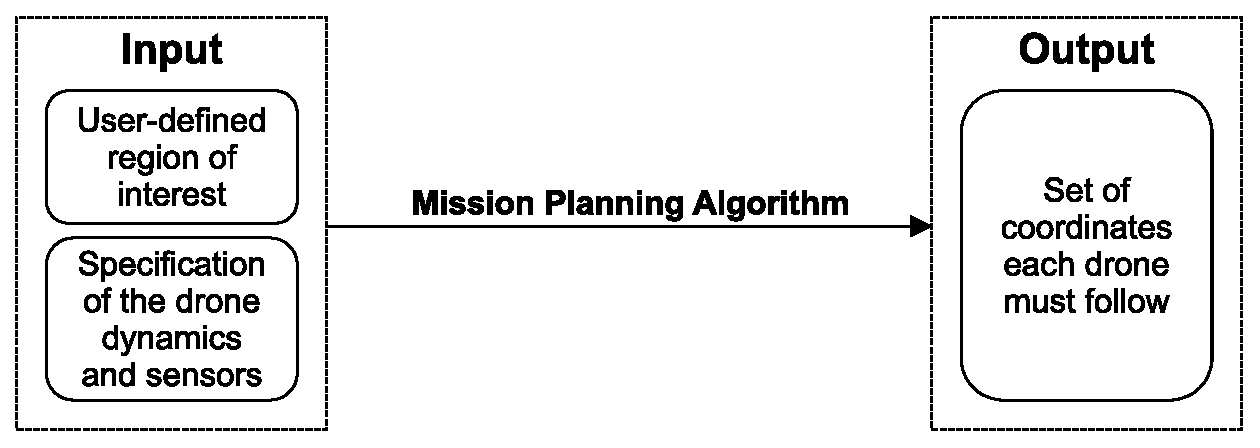
\includegraphics[width=0.7\linewidth]{figs/Jihwan/Objective of the Mission Planning System.eps}
    \caption[Objective of the Mission Planning System]
    {Objective of the mission planning system.}
    \label{fig:msp_objective}
\end{figure}

To have a successful mission planning framework, we wish to meet the following criteria:

\begin{itemize}
    \item \textbf{Efficiency}: The system should be efficient in terms of time, resource and cost compared to previous manual demining methods. 
    \item \textbf{Expandability}: The system should be expandable to a larger area of land by adding additional drones and base stations as necessary. 
    \item \textbf{Intuitiveness}: The system should be easily usable by the members of demining organisations even without professional software knowledge. 
\end{itemize}

This section will explain the theoretical basis of how the mission planning algorithm works for a single-drone system and demonstrate how it meets the criteria above through a real location example. Then, we explain how this algorithm will be expanded into a multi-drone system. Finally, the mission planning algorithm is compared to traditional mine detection methods to evaluate from the criteria above.  

%%%%%%%%%%
\subsection{Layered Approach}
\label{sec:msp_layered_approach}

\subsubsection{Algorithm Outline}

As mentioned in Section~\ref{sensor_hardware_data_acquisition}, we utilise thermal and \gls{GPR} sensors to detect the landmines. Table~\ref{tab:thermal_vs_gpr} illustrates the trade-off between thermal and \gls{GPR} sensors: a thermal sensor is able to scan at a higher altitude and fast speed which results in a shorter time to survey the given \gls{roi}, but a \gls{GPR} sensor results in a higher confidence in the mine location. 

\begin{table}[h!]
    \centering
    \begin{tabular}{| c || c | c |}
        \hline
        Sensor & Thermal & \gls{GPR} \\
        \hline\hline
        Altitude & \textbf{High} & Low \\
        \hline
        Speed & \textbf{Fast} & Slow \\
        \hline
        Confidence & Low & \textbf{High} \\
        \hline
    \end{tabular}
    \caption[Comparison of Thermal and GPR Sensors]
    {Comparison of thermal and \gls{GPR} sensors. Bold entries indicate a comparative advantage.}
    \label{tab:thermal_vs_gpr}
\end{table}

The layered approach aims to optimise between this trade-off by structuring the mission planning algorithm into 6 steps: \textbf{Define}, \textbf{Cover}, \textbf{Analyse}, \textbf{Target}, \textbf{Confirm} and \textbf{Demine}. 

\begin{enumerate}
    \item \textbf{Define}: The \gls{roi} and its obstacles are defined using a \gls{gis} software by the system operator. (Section~\ref{sec:msp_define})
    \item \textbf{Cover}: The \gls{roi} is fully covered by the thermal sensor in a Boustrophedon (back-and-forth) path through a \gls{cpp} algorithm. (Section~\ref{sec:msp_cpp})
    \item \textbf{Analyse}: The resulting thermal sensor readings are analysed by a machine learning algorithm to return a list of suspected landmine points. (Section~\ref{computervision}) 
    \item \textbf{Target}: The suspected landmine points are targeted and rescanned by the \gls{GPR} sensor in a minimum traversal path through a \gls{tspo} algorithm. (Section~\ref{sec:msp_tspo}) 
    \item \textbf{Confirm}: The resulting \gls{GPR} readings are analysed by a machine learning algorithm to return the final result on the locations of the landmines. (Section~\ref{computervision})
    \item \textbf{Demine}: The \gls{roi} is demined based on the generated landmine location map. The demining operation itself is outside the scope of this project, and it will be the responsibility of the demining organisations to safely deactivate and remove the mines.
\end{enumerate}

% add a diagram for summarising the layered approach?

%%%%%%%%%%
\subsection{Defining the Region of Interest}
\label{sec:msp_define}

\subsubsection{Geometric Representation}

The \gls{roi} is an abstract representation of the minefield we wish to survey using our multi-aerial drone system. To apply geometric operations as required by the mission planning algorithm, we represent the \gls{roi} as a Polygon with Holes class (\texttt{Polygon\_with\_holes\_2}) from the \gls{cgal}\footnote{\url{https://www.cgal.org/}} which defines the outer boundary and its holes (obstacles) as a set of vertex coordinates \cite{cgal2024pwh}. \gls{cgal} provides various algorithms that can be directly applied to a Polygon with Holes object -- some of them will be explored and applied in later sections to construct the mission planning algorithm. Throughout the report (Figures \ref{fig:msp_straight_skeleton}, \ref{fig:msp_bahnemann}, \ref{fig:msp_tspo_20_100}, \ref{fig:msp_tspo_plot} and \ref{fig:msp_cdt}), an example Polygon with Holes object extracted from \cite{bahnemann2021cpp} based on a dataset by \cite{sun2014dataset} will be used to represent a simple \gls{roi} with a square outer boundary of width 100\,m. 

\subsubsection{Geographic Information System}

\gls{gis} software connects the geometric representation of the \gls{roi} to a geographic map in an accessible user-interface. This project uses a free and open-source \gls{gis} software called \gls{qgis}\footnote{\url{https://qgis.org/}} from which the demining operator can define the \gls{roi}. The process of defining the \gls{roi} on \gls{qgis} is shown in Figure~\ref{fig:msp_qgis}. Once all the outer polygon and its holes have been created to define the full \gls{roi}, the operator can export the coordinates in a GeoJSON\footnote{\url{https://geojson.org/}} format which gets converted into a Polygon with Holes object.

% add notes on satellite source and mapping drone?

\begin{figure}[h!]
    \centering
    \begin{tabular}{cc}
        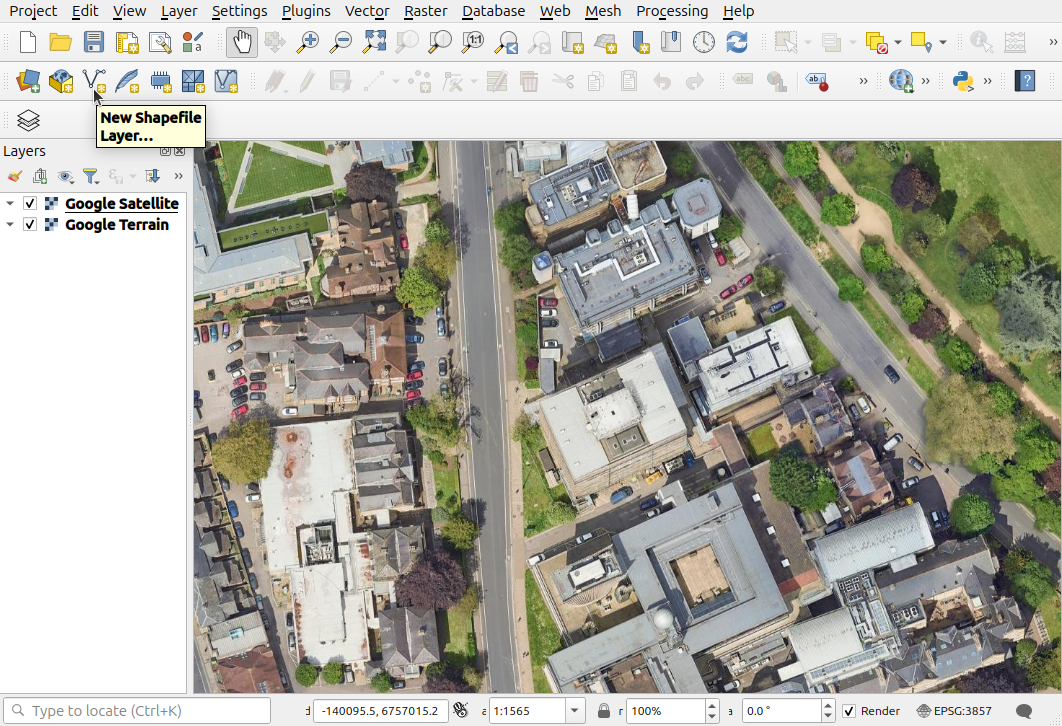
\includegraphics[width=0.45\textwidth]{figs/Jihwan/qgis_a.png} &
        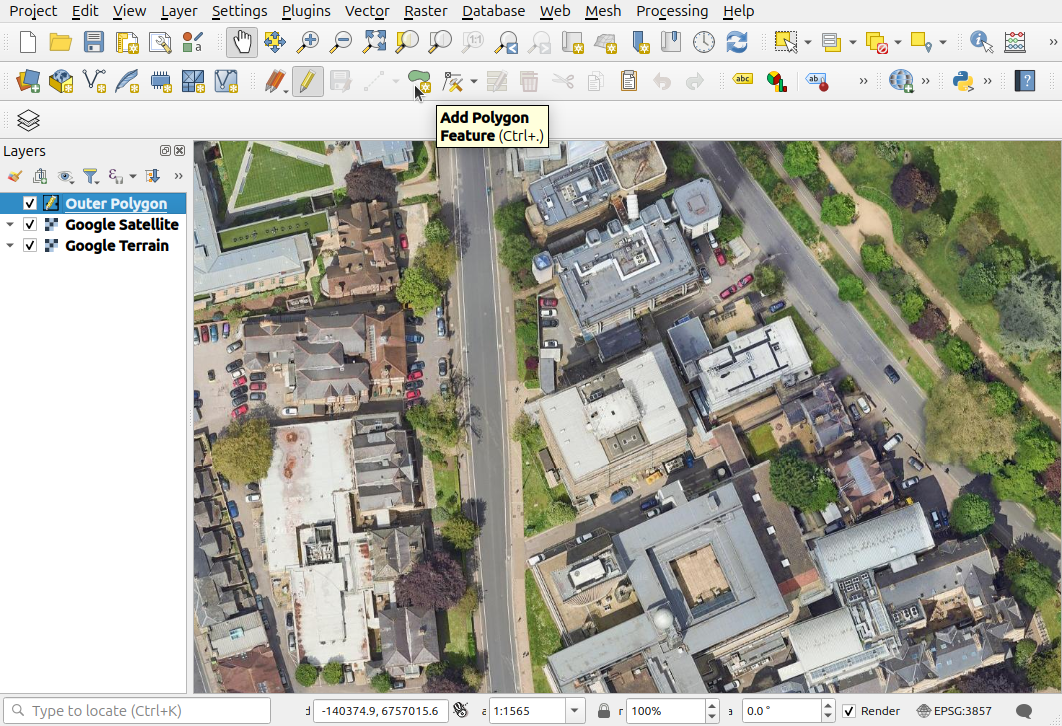
\includegraphics[width=0.45\textwidth]{figs/Jihwan/qgis_b.png} \\
        (a) & (b) \\[10pt]
        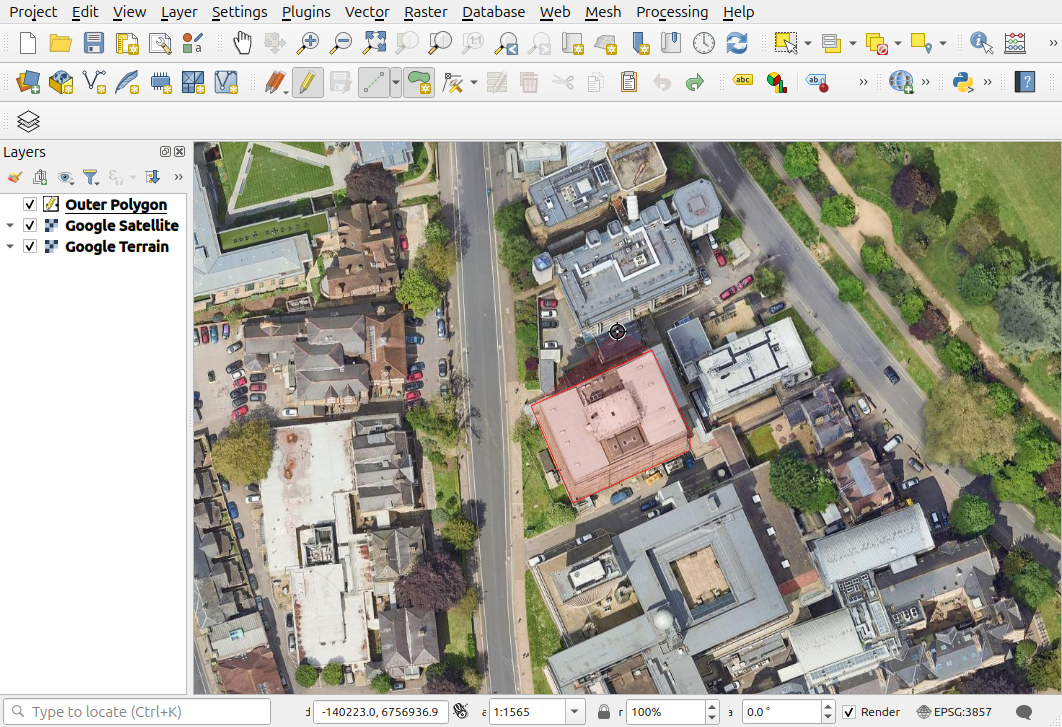
\includegraphics[width=0.45\textwidth]{figs/Jihwan/qgis_c.png} &
        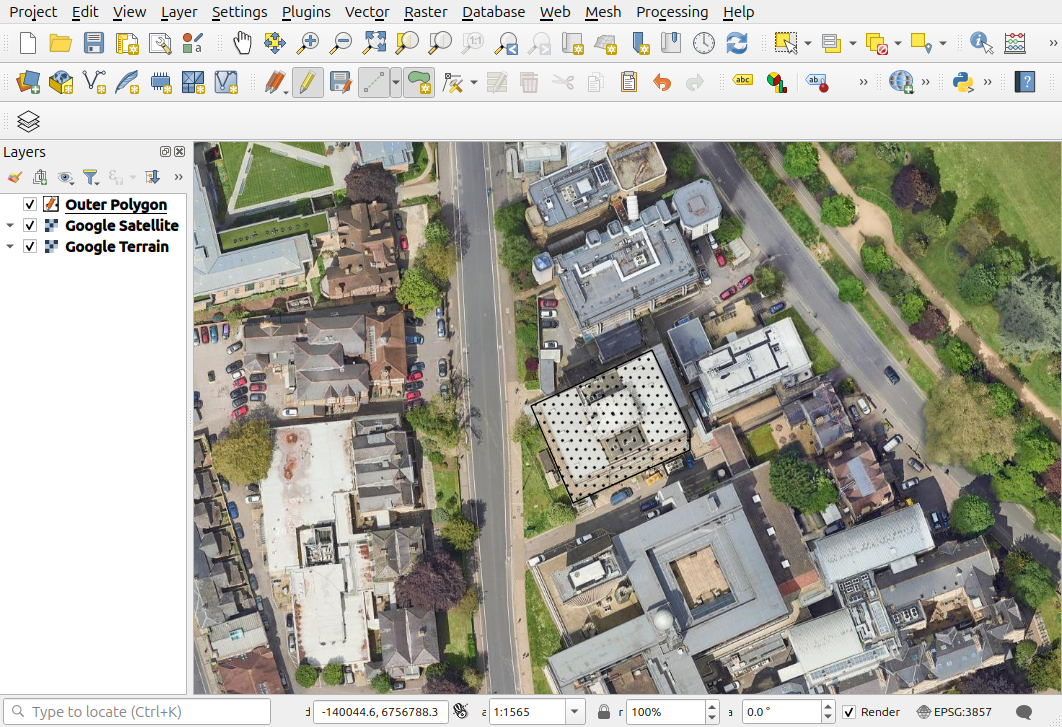
\includegraphics[width=0.45\textwidth]{figs/Jihwan/qgis_d.png} \\
        (c) & (d)
    \end{tabular}
    \caption[Demonstration of ROI Definition using QGIS]
    {Demonstration of defining the \gls{roi} using \gls{qgis}. (a) New Shapefile layer is created. (b) New polygon feature named "Outer Polygon" is defined. (c) The system operator marks the vertices of the polygon. (d) The final polygon is displayed. Additional polygons can be added to define the full \gls{roi}.}
    \label{fig:msp_qgis}
\end{figure}

% add note on coordinate system? qgis uses epsg:3857 but it can be changed. 

\subsubsection{Boundary Offset}

In some cases, it may be necessary to ensure that the drones do not exit the \gls{roi} or approach any of its internal obstacles. To do so, a boundary offset can be introduced using the straight skeleton algorithm as suggested in \cite{shahid2024cpp}. The straight skeleton of a polygon can be found by a shrinking process in which the boundary is contracted towards the interior in a self-parallel manner and at the same speed for all edges \cite{aichholzer1996ss}. Applying the shrinking process by a specified length would result in an internal boundary offset of the original polygon. \gls{cgal} provides an implementation for the straight skeleton algorithm in its 2D Straight Skeleton and Polygon Offsetting package which can be directly applied to a Polygon with Holes object \cite{cgal2024ss}.

Figure~\ref{fig:msp_straight_skeleton} shows the result of applying \gls{cgal}'s straight skeleton algorithm to obtain the offset of the \gls{roi} boundary. It shows a successful generation of the boundary offset even for complex geometries, validating this approach for the use case. Furthermore, the size of the offset can be varied depending on the requirements of the mission. 

\begin{figure}[h!]
    \centering
    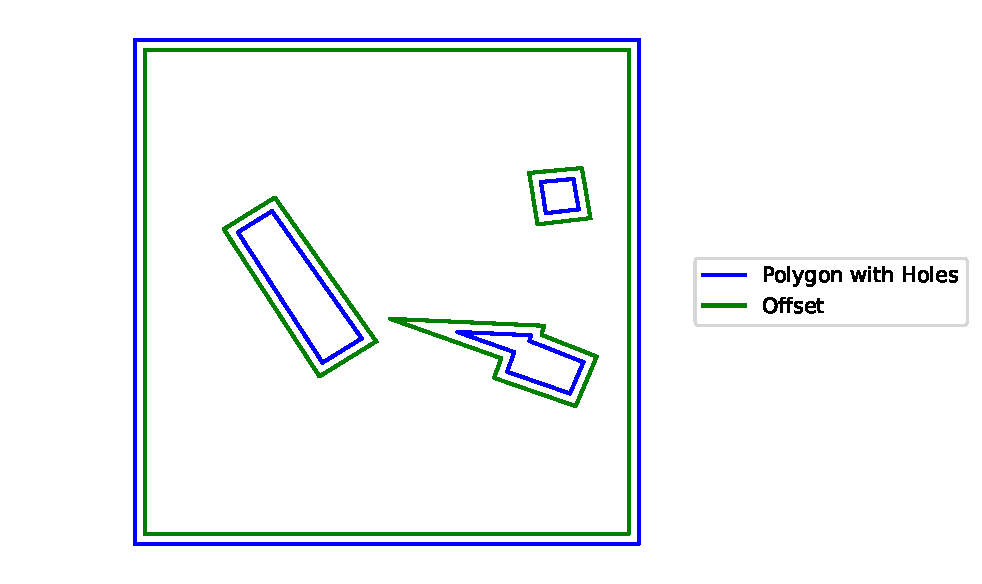
\includegraphics[width=0.6\linewidth]{figs/Jihwan/Polygon Offset with Straight Skeleton.pdf}
    \caption[Offset of ROI using Straight Skeleton]
    {A 2\,m offset of a Polygon with Holes has been generated using \gls{cgal}'s straight skeleton method.}
    \label{fig:msp_straight_skeleton}
\end{figure}

%%%%%%%%%%
\subsection{Coverage Path Planning}
\label{sec:msp_cpp}

\gls{cpp} is a task in which an agent (drone) must cover every point in the given environment (\gls{roi}) with its method of action (thermal sensor reading). To obtain the solution of a \gls{cpp} problem, the \gls{roi} is first decomposed into smaller polygons. In large, this can be distinguished between \textit{approximate} and \textit{exact} cellular decompositions. In an approximate cellular decomposition the \gls{roi} is decomposed into a grid of same size and shape (often a square). Assuming that a single grid is smaller than the size of the sensor's field of view, visiting all grids would indicate a full coverage of the \gls{roi} except the areas which are lost during the approximation process. In contrast, an exact cellular decomposition divides the \gls{roi} into a set of non-intersecting cells which are covered by a continuous path of motion, covering the entire \gls{roi} without missing regions \cite{choset2001surveycpp}. 

For the purpose of a landmine detection system, it is important to use the exact cellular decomposition. This would ensure that no landmines that could cause a safety hazard for the demining individuals have been missed out. In particular, this project uses the \gls{bcd} and path planning method that has been implemented by \cite{bahnemann2021cpp} which will be explained in detail below.  

\subsubsection{Boustrophedon Cellular Decomposition and Path Planning}

\gls{bcd} is an exact cellular decomposition method first proposed by \cite{choset1998bcd}. It stems from \gls{tcd} -- a straight line segment sweeps through the decomposition area in one direction, dividing the area into trapezoidal cells each time it passes through a vertex of the obstacle polygons (Figure~\ref{fig:msp_choset}a). \gls{bcd} reduces the number of cells created by merging trapezoidal cells which occur between \textit{IN} (the straight line segmented is divided into two by the obstacle) and \textit{OUT} (the straight line segments are merged into one after passing the obstacle) events (Figure~\ref{fig:msp_choset}b). Having a fewer number of cells helps avoid unnecessary overlapping swaths from being generated in between two neighbouring cells as demonstrated in Figure~\ref{fig:msp_choset}c. 

\begin{figure}[h!]
    \centering
    \begin{tabular}{p{0.3\textwidth}p{0.3\textwidth}p{0.3\textwidth}}
        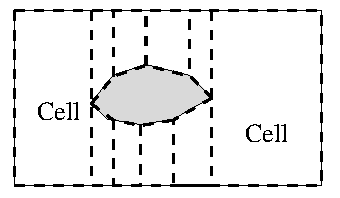
\includegraphics[width=0.3\textwidth]{figs/Jihwan/choset_tcd.pdf} &
        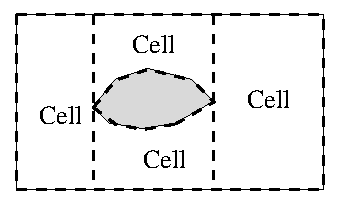
\includegraphics[width=0.3\textwidth]{figs/Jihwan/choset_bcd.pdf} &
        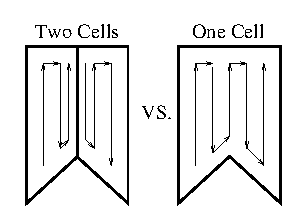
\includegraphics[width=0.3\textwidth]{figs/Jihwan/choset_bcd_tcd_comparison.pdf} \\
        \centering (a) Resulting cells from \gls{tcd} giving 10 cells. & 
        \centering (b) Resulting cells from \gls{bcd} giving 4 cells. & 
        \centering (c) Comparison of coverage paths using \gls{tcd} (left) and \gls{bcd} (right).
    \end{tabular}
    \caption[Comparison between TCD and BCD]
    {Comparison between \gls{tcd} and \gls{bcd} adapted from \cite{choset1998bcd}.}
    \label{fig:msp_choset}
\end{figure}

In each cell, boustrophedon (back-and-forth) paths are generated for the drone to cover the region with its sensor. Based on the thermal sensor decided in Section~\ref{thermal_system}, the coverage width of the drone travelling in a straight line is approximately 9\,m. A set of parallel lines are drawn within the boundary of the cell with spacings equal to the coverage width. The end of these parallel lines are then connected appropriately to generate the continuous path the drone must take to fully cover the cell with its sensor's \gls{FOV}. Based on the angle at which the parallel lines are drawn, the coverage path can be optimised with respect to two different loss functions: the total distance travelled or the number of turns taken (as turning is a costly manoeuvrer compared to a straight path, so it should be minimised). The method for finding the optimal angle for convex and non-convex polygons is discussed in \cite{torres2016cpp} which in brief involves finding the maximum width of the cell's convex hull. 

The boustrophedon paths of each cell should now be connected to form a continuous path across all cells in the decomposition. This can be done by the use of an adjacency graph \cite{choset1998bcd}. An undirected graph is initialised where each cell of the decomposition corresponds to a node. Edges are created between cells which are adjacent to one another (two cells share one or more edges) where the weight is the distance between the end of one cell's coverage path to the start of the other cell's coverage path. The \gls{cpp} problem is now simplified into one in which the agent (drone) must visit all cells in the adjacency graph at least once, covering each cell with their individual boustrophedon paths. This is equivalent to a \gls{tsp}, for which the solutions will be explored in more detail in Section~\ref{sec:msp_tspo}. 

In the end, we are able to find a continuous path for the drone which is able to cover the entire \gls{roi}. The whole \gls{cpp} algorithm explained above is well-summarised by Figure~\ref{fig:msp_cabreira} from \cite{cabreira2019surveycpp}, which shows the full example of generating the coverage path of a \gls{roi} without any obstacles. The procedure for a \gls{roi} with obstacles is similar except for the fact that the connecting paths in between the cells may need to go around the obstacles.  

\begin{figure}[h!]
    \centering
    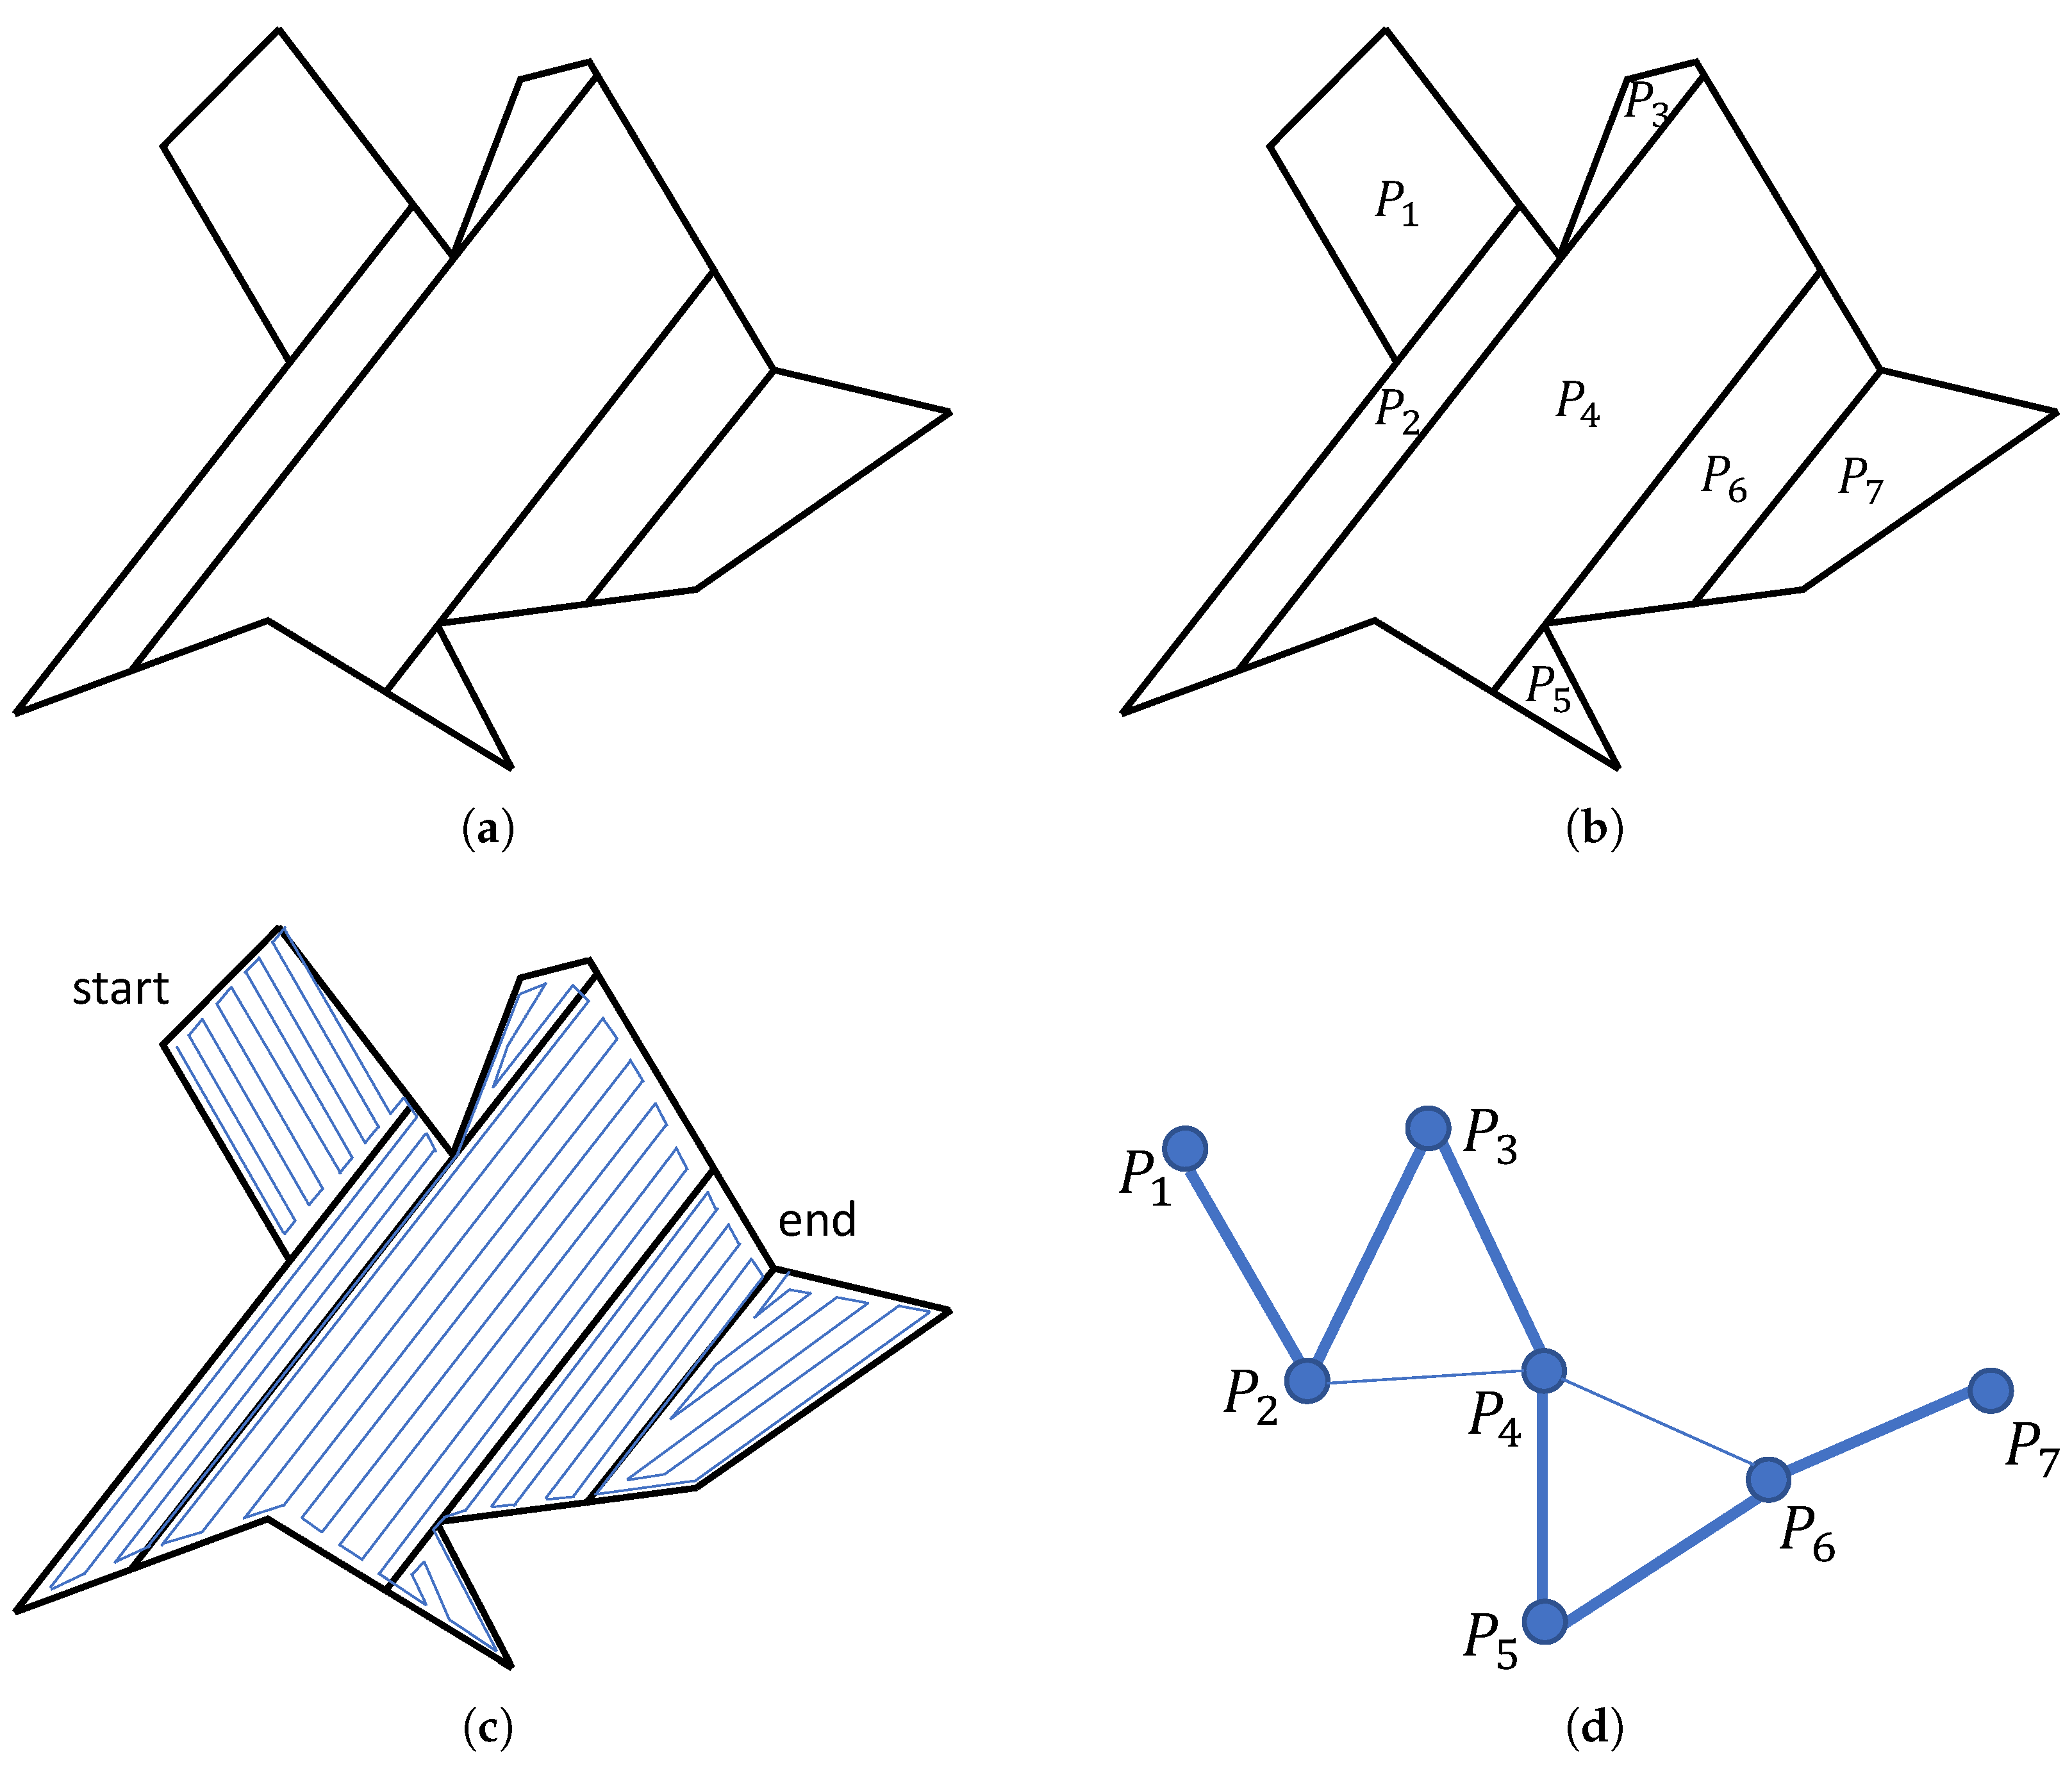
\includegraphics[width=0.7\linewidth]{figs//Jihwan/cabreira.png}
    \caption[Example of the Full CPP Algorithm]{Example of the full \gls{cpp} algorithm by \cite{cabreira2019surveycpp}. (a) The \gls{roi} is decomposed using \gls{bcd}. (b) Each cell is assigned as a node in the adjacency graph. (c) The boustrophedon paths of each cell is generated and connected based on the \gls{tsp} solution of the adjacency graph. (d) The \gls{tsp} solution of the adjacency graph is shown for clarity.}
    \label{fig:msp_cabreira}
\end{figure}

\subsubsection{Implementation}

To solve the \gls{cpp} problem, an implementation made by \cite{bahnemann2021cpp} (available on their GitHub repository ethz-asl/polygon\_coverage\_planning\footnote{\url{https://github.com/ethz-asl/polygon_coverage_planning/tree/master}}) is used. The program is subject to the GNU GPL-3.0 license\footnote{\url{https://www.gnu.org/licenses/gpl-3.0.en.html}} allowing commercial uses of copy, modification and distribution of the software given that it is subject to the same license. 

For use, the software must be compiled from its ROS Noetic\footnote{\url{https://wiki.ros.org/noetic}} packages on the Ubuntu 20.04 operating system. It allows for flexible customisation of the \gls{roi} as well as sensor specifications (drone height, sensor FOV angle, sensor coverage width, etc.) through the configuration files which can be run as ROS server requests. The output broadcasts the coverage path the drone must take in Cartesian coordinates, which can be converted and returned to the \gls{qgis} interface for approval by the demining operator. Figure~\ref{fig:msp_bahnemann} demonstrates the \gls{cpp} solutions for different sensor coverage widths found using the program. 

\begin{figure}[h!]
    \centering
    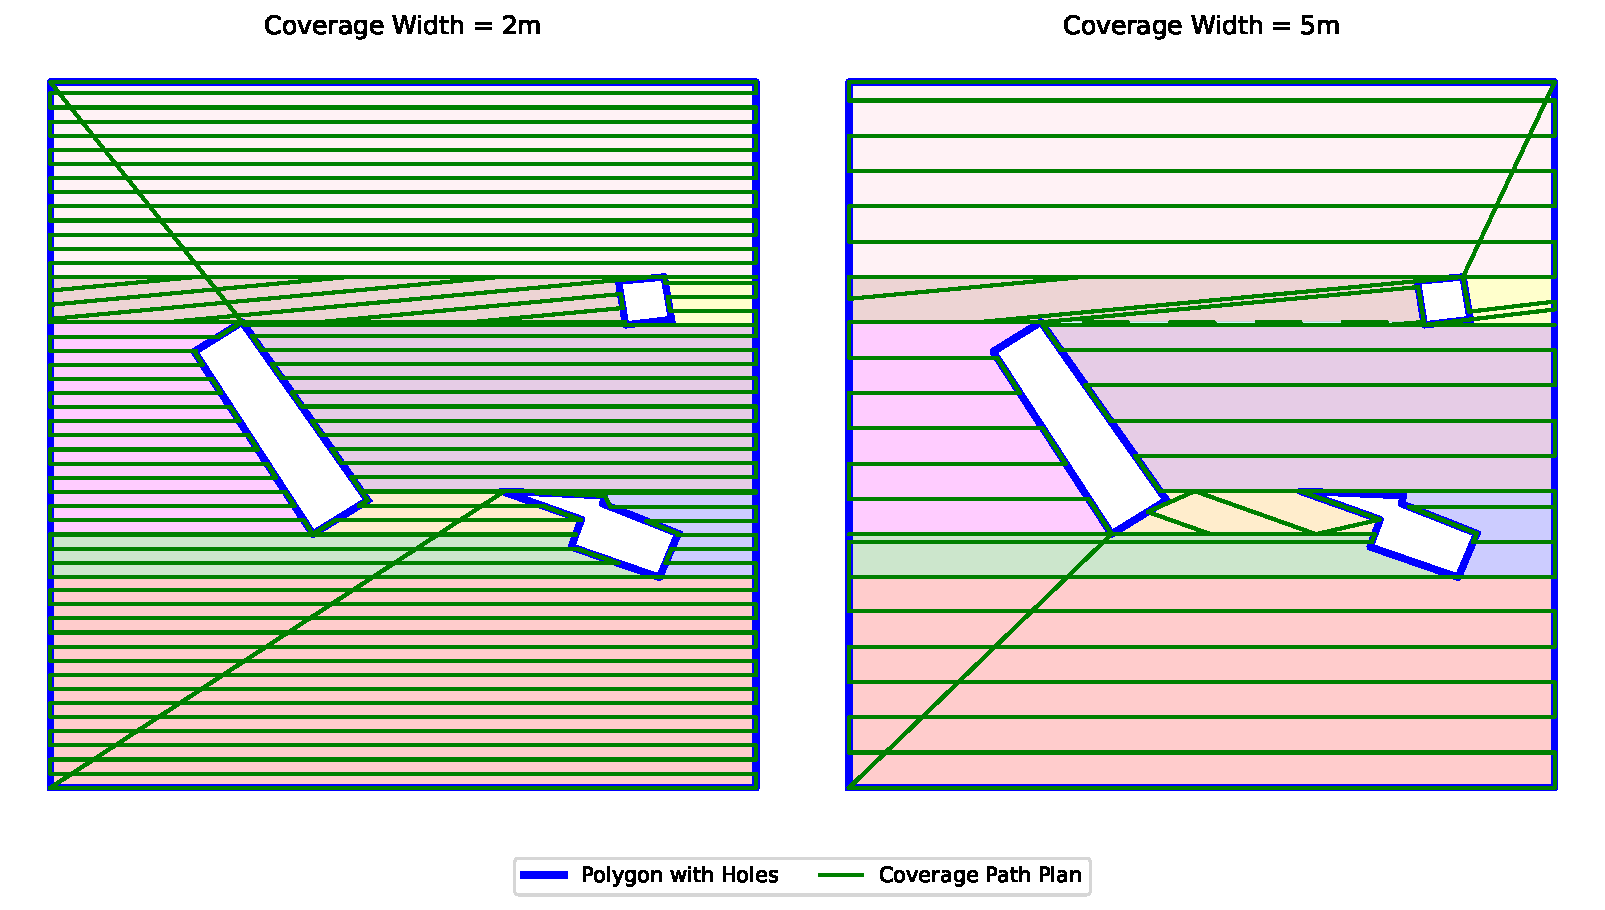
\includegraphics[width=\linewidth]{figs/Jihwan/CPP_diff_widths.pdf}
    \caption[CPP Solution Examples]
    {\gls{cpp} solutions have been found for sensor coverage widths of 2\,m (left) and 5\,m (right). The colour of the background indicates segmentations resulting from the \gls{bcd}.}
    \label{fig:msp_bahnemann}
\end{figure}

In this project, the software was compiled in a virtual machine (Multipass\footnote{\url{https://canonical.com/multipass}} Ubuntu 20.04 with NoMachine\footnote{\url{https://www.nomachine.com/}}) installed in an Ubuntu 24.01 host computer. The computational requirement of the software was sufficient to be run with this method, but in a real scenario it may be beneficial to port over the software as ROS2 Jazzy\footnote{\url{https://docs.ros.org/en/jazzy/index.html}} packages which can be run locally in the Ubuntu 24.01 host computer for a better integration with \gls{qgis} as well as other components of the layered approach. 

%%%%%%%%%%
\subsection{Travelling Salesman Problem with Obstacles}
\label{sec:msp_tspo}

\subsubsection{Travelling Salesman Problem}

The \gls{tsp} is an optimisation problem in which the minimum traversal path to visit all targeted nodes in a weighted graph must be found. A number of exact (optimal) and heuristic solutions have been studied and proposed as reviewed in \cite{laporte1992tsp} and \cite{zhang2023tsp}. Some of the methods have been compiled and compared in Table~\ref{tab:msp_tspcomparison}.  

\begin{table}[h!]
    \centering
    \begin{tabular}{|c|p{0.5\linewidth}|c|}
        \hline
        \textbf{Method} & \centering{\textbf{Explanation}} & \textbf{Complexity} \\
        \hline \hline
        Brute-Force Algorithm & Naïve method where all possible permutations are calculated to find the optimal solution. & $O(n!)$ \\ \hline
        Held-Karp Algorithm \cite{held1962hktsp} & Dynamic Programming method where subsets of nodes are explored to find the optimal solution. It improves on the brute-force method in terms of complexity while maintaining the optimal solution, but comes at the cost of large memory requirements. & $O(n^2 2^n)$ \\ \hline
        Genetic Algorithm \cite{potvin1996gentsp} & Searches for the heuristic solution by combining the best features of good solutions over multiple generations. & $O(n^2 g)$ \\ \hline
        Ant Colony Optimisation \cite{dorigo1997anttsp} & Mimics the behaviour of ants leaving pheromone trail (on edges of the graph) to successively shorten the path for a heuristic solution. & $O(n^2 m)$ \\ \hline
        Lin-Kernighan Algorithm \cite{lin1973lktsp} & Iteratively swap edges for local optimisation to find the heuristic solution. It is a popularly used method due to its performance and efficiency. & $O(n^2\log{n})$ \\ \hline
    \end{tabular}
    \caption[Comparison of TSP Solution Methods]
    {A comparison of \gls{tsp} solution methods. The complexity is expressed using Big O notation for the following variables: $n$ (number of nodes), $g$ (number of generations), $m$ (number of ants per iteration). The complexity may vary depending on the implementation.}
    \label{tab:msp_tspcomparison}
\end{table}

For the purpose of our layered approach, the number of suspected points will get large due to the size of the \gls{roi} and leniency towards high recall for the thermal sensor analysis algorithm (Section~\ref{compvis_intro}). It is also acceptable to sacrifice the optimality of the solution as it is not critical for surveying the \gls{roi} with the \gls{GPR} sensor. Hence, we choose the heuristic Lin-Kernighan algorithm for our problem. 

% more detailed explanation of the lk algorithm? 

The \gls{tsp} can be extended to more specific cases depending on the application, one of which is the \gls{tspo}. It introduces obstacles which the traversal path must avoid; this is exactly the problem that must be solved for the Target step of the layered approach, as the drone with a \gls{GPR} sensor must visit all suspected landmine points in the obstacle-filled \gls{roi}. The method for solving \gls{tspo} is explained in the next section. 

\subsubsection{Solving TSP-O using Visibility Graph}

One of the methods of solving a \gls{tspo} is to convert it into an ordinary \gls{tsp} using visibility graphs. A visibility graph is a data structure in which two nodes that are \textit{visible} (i.e. straight line segment between two nodes is not obstructed by any obstacles) are connected by an edge. In the context of geometric application like this project, the weight of the edge is defined to be the Euclidean distance between them. To check the visibility between two nodes on the 2D plane, \gls{cgal}'s 2D Visibility package \cite{cgal2024visibility} provides an implementation of the triangular expansion algorithm which can be applied on a Polygon with Holes object. By creating a visibility graph where all vertices of the \gls{roi} and the suspected landmine points are the nodes with visibility edges connecting them, the \gls{tspo} is simplified into an ordinary \gls{tsp} that can be solved using the \gls{tsp} solution listed in the previous section. This idea is explored in \cite{barb2024tspo} and \cite{bhat2024tspo} for more specific applications. 

The algorithm for converting a \gls{tspo} into a visibility graph given the Polygon with Holes $P$ and suspected (target) points $T$ is explained as pseudocode in Algorithm~\ref{alg:msp_tspo2visgraph}. It returns the visibility graph representation of the \gls{tspo}. The full process for solving the \gls{tspo} is visualised with a simple example in Figure~\ref{fig:msp_tspo}.

\begin{algorithm}[h!]
\caption{Creating the Visibility Graph of \gls{tspo}}
\label{alg:msp_tspo2visgraph}
\begin{algorithmic}[1]
\Require Polygon with Holes $P$, Set of target points $T = \{t_1, t_2, \ldots, t_q\}$ within $P$
\Ensure Visibility graph $G = (V, E)$

\State Initialize visibility graph $G = (V, E)$ with $V = \emptyset$ and $E = \emptyset$
\State $V \leftarrow T$ \Comment{Add all target points to the graph}
\State $V \leftarrow V \cup \text{Vertices}(P)$ \Comment{Add all vertices of polygon with holes to the graph}

\ForAll{$u \in V$}
    \ForAll{$v \in V$ where $u \neq v$}
        \If{$\text{IsVisible}(u, v)$}
            \State $E \leftarrow E \cup \{(u, v, d(u, v))\}$ \Comment{Add edge with Euclidean distance weight}
        \EndIf
    \EndFor
\EndFor

\Return $G$ \Comment{Return visibility graph}
\end{algorithmic}
\end{algorithm}

\begin{figure}[h!]
    \centering
    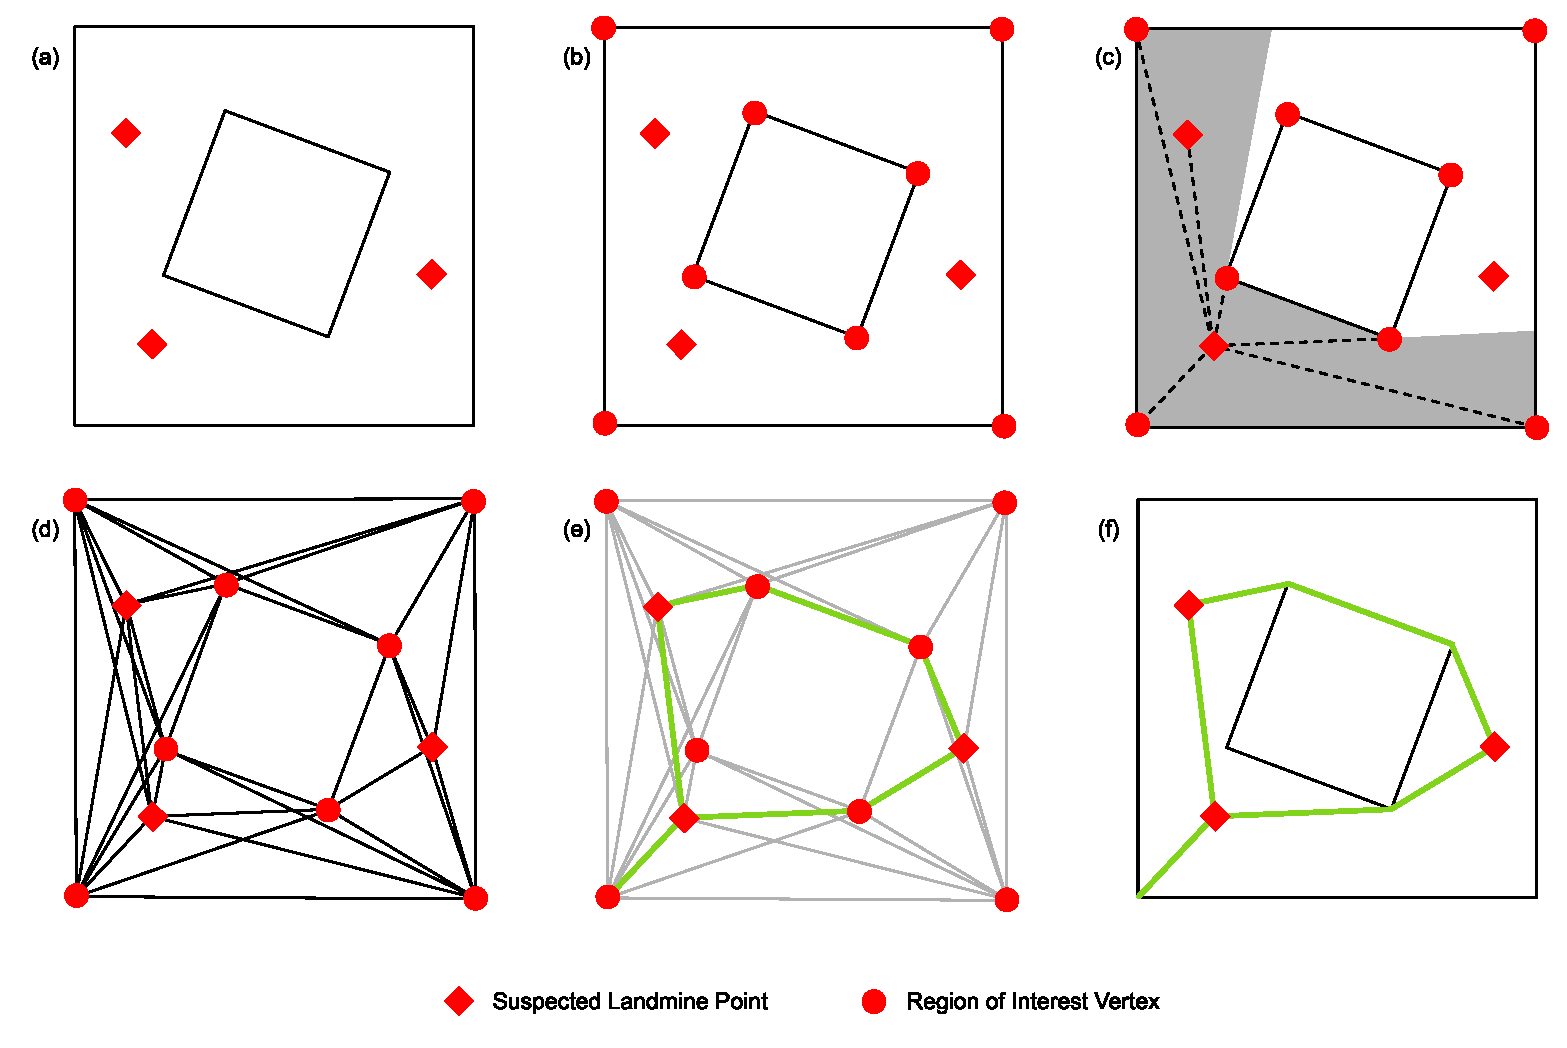
\includegraphics[width=\linewidth]{figs/Jihwan/TSPO Algorithm Visualisation.eps}
    \caption[TSP-O Algorithm Visualisation]
    {\gls{tspo} algorithm visualisation. (a) The example \gls{roi} is defined to have an outer boundary (outer square) with an obstacle (rotated inner square). Assume three suspected landmine points have been found from the Analyse step. (b) Add all suspected landmine points and \gls{roi} vertices as nodes to the visibility graph. (c) For each node, examine which other nodes are visible. Grey area indicates the visible region of the lower-left suspected landmine point. (d) Add weighted edges between visible nodes, with the weight being the Euclidean distance between them. The figure shows all connected edges between all nodes. (e) Perform a \gls{tsp} algorithm to visit all suspected landmine points in the visibility graph, starting from and ending at the base station. In this example, the lower left vertex of the outer boundary is defined as the base station. (f) Final solution of the minimal traversal path to visit all suspected landmine points is displayed, solving the \gls{tspo} algorithm. 
    }
    \label{fig:msp_tspo}
\end{figure}

\subsubsection{Time Complexity}

The time complexity of algorithm~\ref{alg:msp_tspo2visgraph} can be calculated to estimate the computing requirements for solving the \gls{tspo}. Note that the visibility condition is checked through the IsVisible($u$,$v$) function which is inside two nested for-loops iterating through all nodes in the visibility graph. Let $n$ be the number of nodes, which is equal to the sum of $p$ (the number of vertices in $P$) and $q$ (the number of points in $T$). In addition, let $h$ be the number of holes + 1. According to \cite{cgal2024visibility}, the time complexity for \gls{cgal}'s implementation of the visibility check (triangular expansion algorithm) is $O(n h)$. The nested for-loops will multiply $O(n)$ to the time complexity twice. Hence, the worst-case time complexity of Algorithm~\ref{alg:msp_tspo2visgraph} can be expressed as $O(n^3 h)$. 

The resulting visibility graph is then solved as an ordinary \gls{tsp} through the use of Lin-Kernighan algorithm explained above, which has the time complexity $O(n^2\log{n})$. Algorithm~\ref{alg:msp_tspo2visgraph} and the Lin-Kernighan algorithm are applied successively, meaning that their time complexities will be added to give $O(n^3 h + n^2\log{n})$. 

As $n$ increases to a large value, $O(n^2\log{n})$ becomes negligible compared to $O(n^3 h)$ in terms of its magnitude. The final time complexity of finding the solution to \gls{tspo} can therefore be expressed as $O(n^3 h)$. This is a reasonable value for computation given that the number of suspected landmine points does not come out to be too high for the \gls{roi}. 

% it will get too high, so we divide and cluster. 

\subsubsection{Implementation}

The \gls{tspo} was implemented using C++ based on the algorithms explained above, which gives the heuristic solution that cycles around the target points within a Polygon with Holes object. Figure~\ref{fig:msp_tspo_20_100} shows the computed solution for 20 and 100 randomly generated target points. They show near-optimal tour path confirming the validity of the implementation, exhibiting a behaviour in which the path wraps around the obstacles where necessary to achieve the minimum distance. This behaviour re-emphasises the need of a straight skeleton algorithm. 

Figure~\ref{fig:msp_tspo_plot} shows the effect of the number of target points on the computing time and total travel distance. The computing time rapidly increases as the number of target points passes 100 -- if the estimated computing time becomes too large, the operator may choose to divide the \gls{roi} into smaller subregions to reduce the total computing time. This would introduce an inefficiency in the total distance travelled by the drones, but it may become necessary due to the constraint of how much distance a single drone can cover before recharging. 

% add notes on how the implementation is sub-optimal and how it can be improved? would need to explain lin-kernighan in more detail first. 

\begin{figure}[h!]
    \centering
    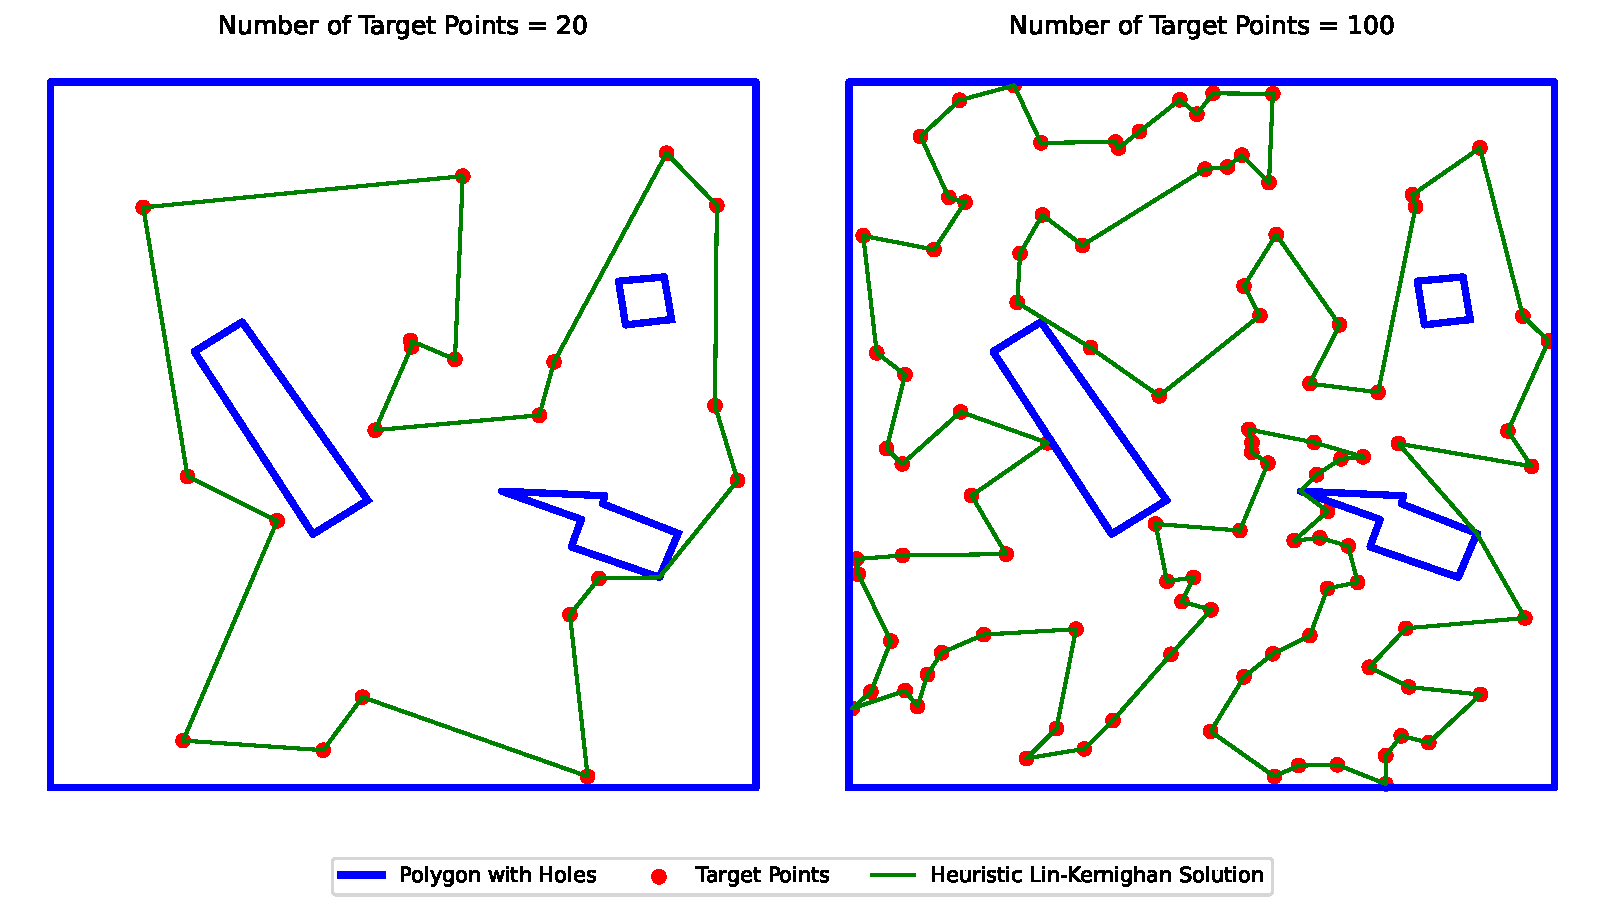
\includegraphics[width=\linewidth]{figs/Jihwan/TSPO_diff_targets.pdf}
    \caption[TSP-O Solution for Different Numbers of Target Points]
    {\gls{tspo} solutions have been generated for 20 (left) and 100 (right) target points randomly generated through rejection sampling.}
    \label{fig:msp_tspo_20_100}
\end{figure}

\begin{figure}[h!]
    \centering
    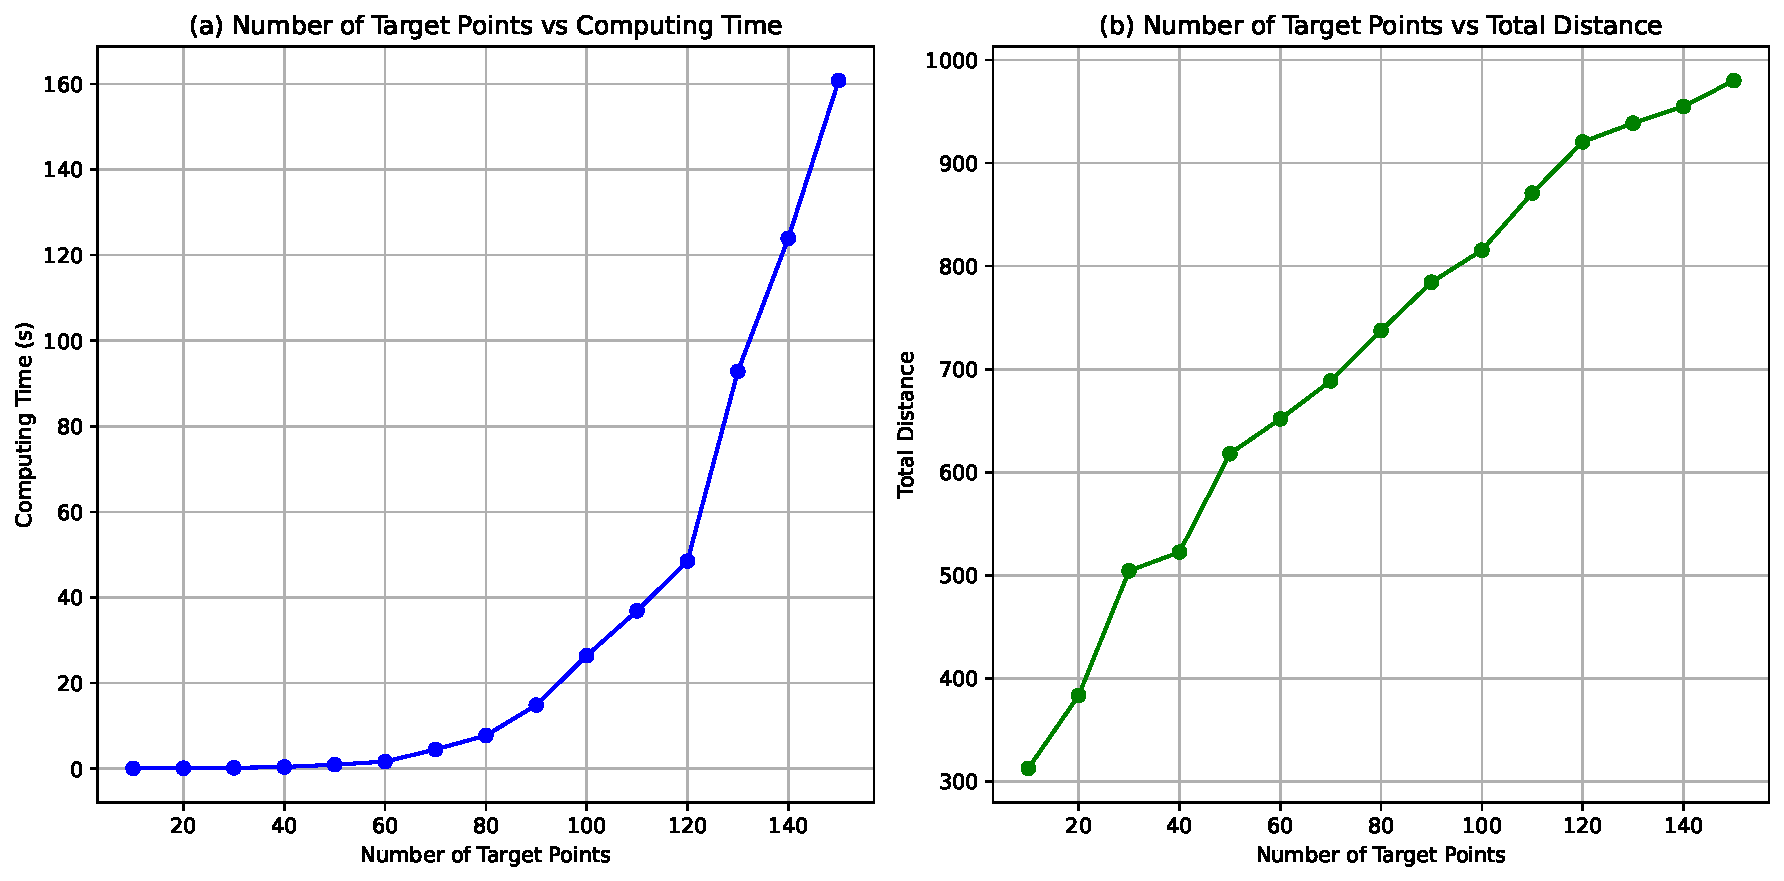
\includegraphics[width=\linewidth]{figs/Jihwan/target_points_vs.pdf}
    \caption[Effect of Number of Target Points on Computing Time and Total Distance of TSP-O Solution]
    {Plots showing the effect of the number of target points on the computing time (left) and total distance (right) in \gls{tspo}. Number of Target Points have been changed from 10 to 150 at increments of 10, taking the mean of 3 trials each where the target points are randomly generated through rejection sampling. The total distance is based on the scale where the width of the outer boundary is 100\,m.}
    \label{fig:msp_tspo_plot}
\end{figure}

%%%%%%%%%%
\subsection{Real Location Example}
\label{sec:msp_example}

To test the validity of the layered approach, a real location example has been conducted for an arbitrarily selected \gls{roi} at Ukraine (51°20'22.1"N 29°56'48.8"E) shown in Figure~\ref{fig:msp_example}a. The example demonstrates the Define, Cover and Target steps of the layered approach by displaying the results of each step on \gls{qgis}. 

\paragraph{Define} Figure~\ref{fig:msp_example}b shows the \gls{roi} defined using \gls{qgis}. The \gls{roi} is about the size of a 400\,m by 400\,m field with 3 obstacles which have been manually identified.  

\paragraph{Cover} Figure~\ref{fig:msp_example}c shows the \gls{cpp} solution found using the implementation by \cite{bahnemann2021cpp}. The coverage width has been specified as approximately 9\,m, and the start/end points have been arbitrarily decided to be at the top-right region outside the \gls{roi}. A thermal sensor drone will follow the generated path plan to collect the thermal readings. The total length of the path is calculated to be 15526\,m.

\paragraph{Target} Figure~\ref{fig:msp_example}d shows the \gls{tspo} solution found using Algorithm~\ref{alg:msp_tspo2visgraph} and the heuristic Lin-Kernighan algorithm. To represent the suspected landmine points, 20 coordinates within the \gls{roi} have been randomly generated using rejection sampling. The total length of the path is calculated to be 1777\,m. In a real mission, the suspected landmine points would be found during the Analyse step based on the thermal readings. At each point, the \gls{GPR} sensor drone will perform the scanning procedure described in Section~\ref{GPR_flight} before continuing onto the next point. 

For Cover and Target, if the total length of the path is too large to be covered by a single drone the operator may choose to deploy multiple drones to cover the \gls{roi}. This is further explained in Section~\ref{sec:msp_multi_drone}. 

\begin{figure}[h!]
    \centering
    \begin{tabular}{cc}
        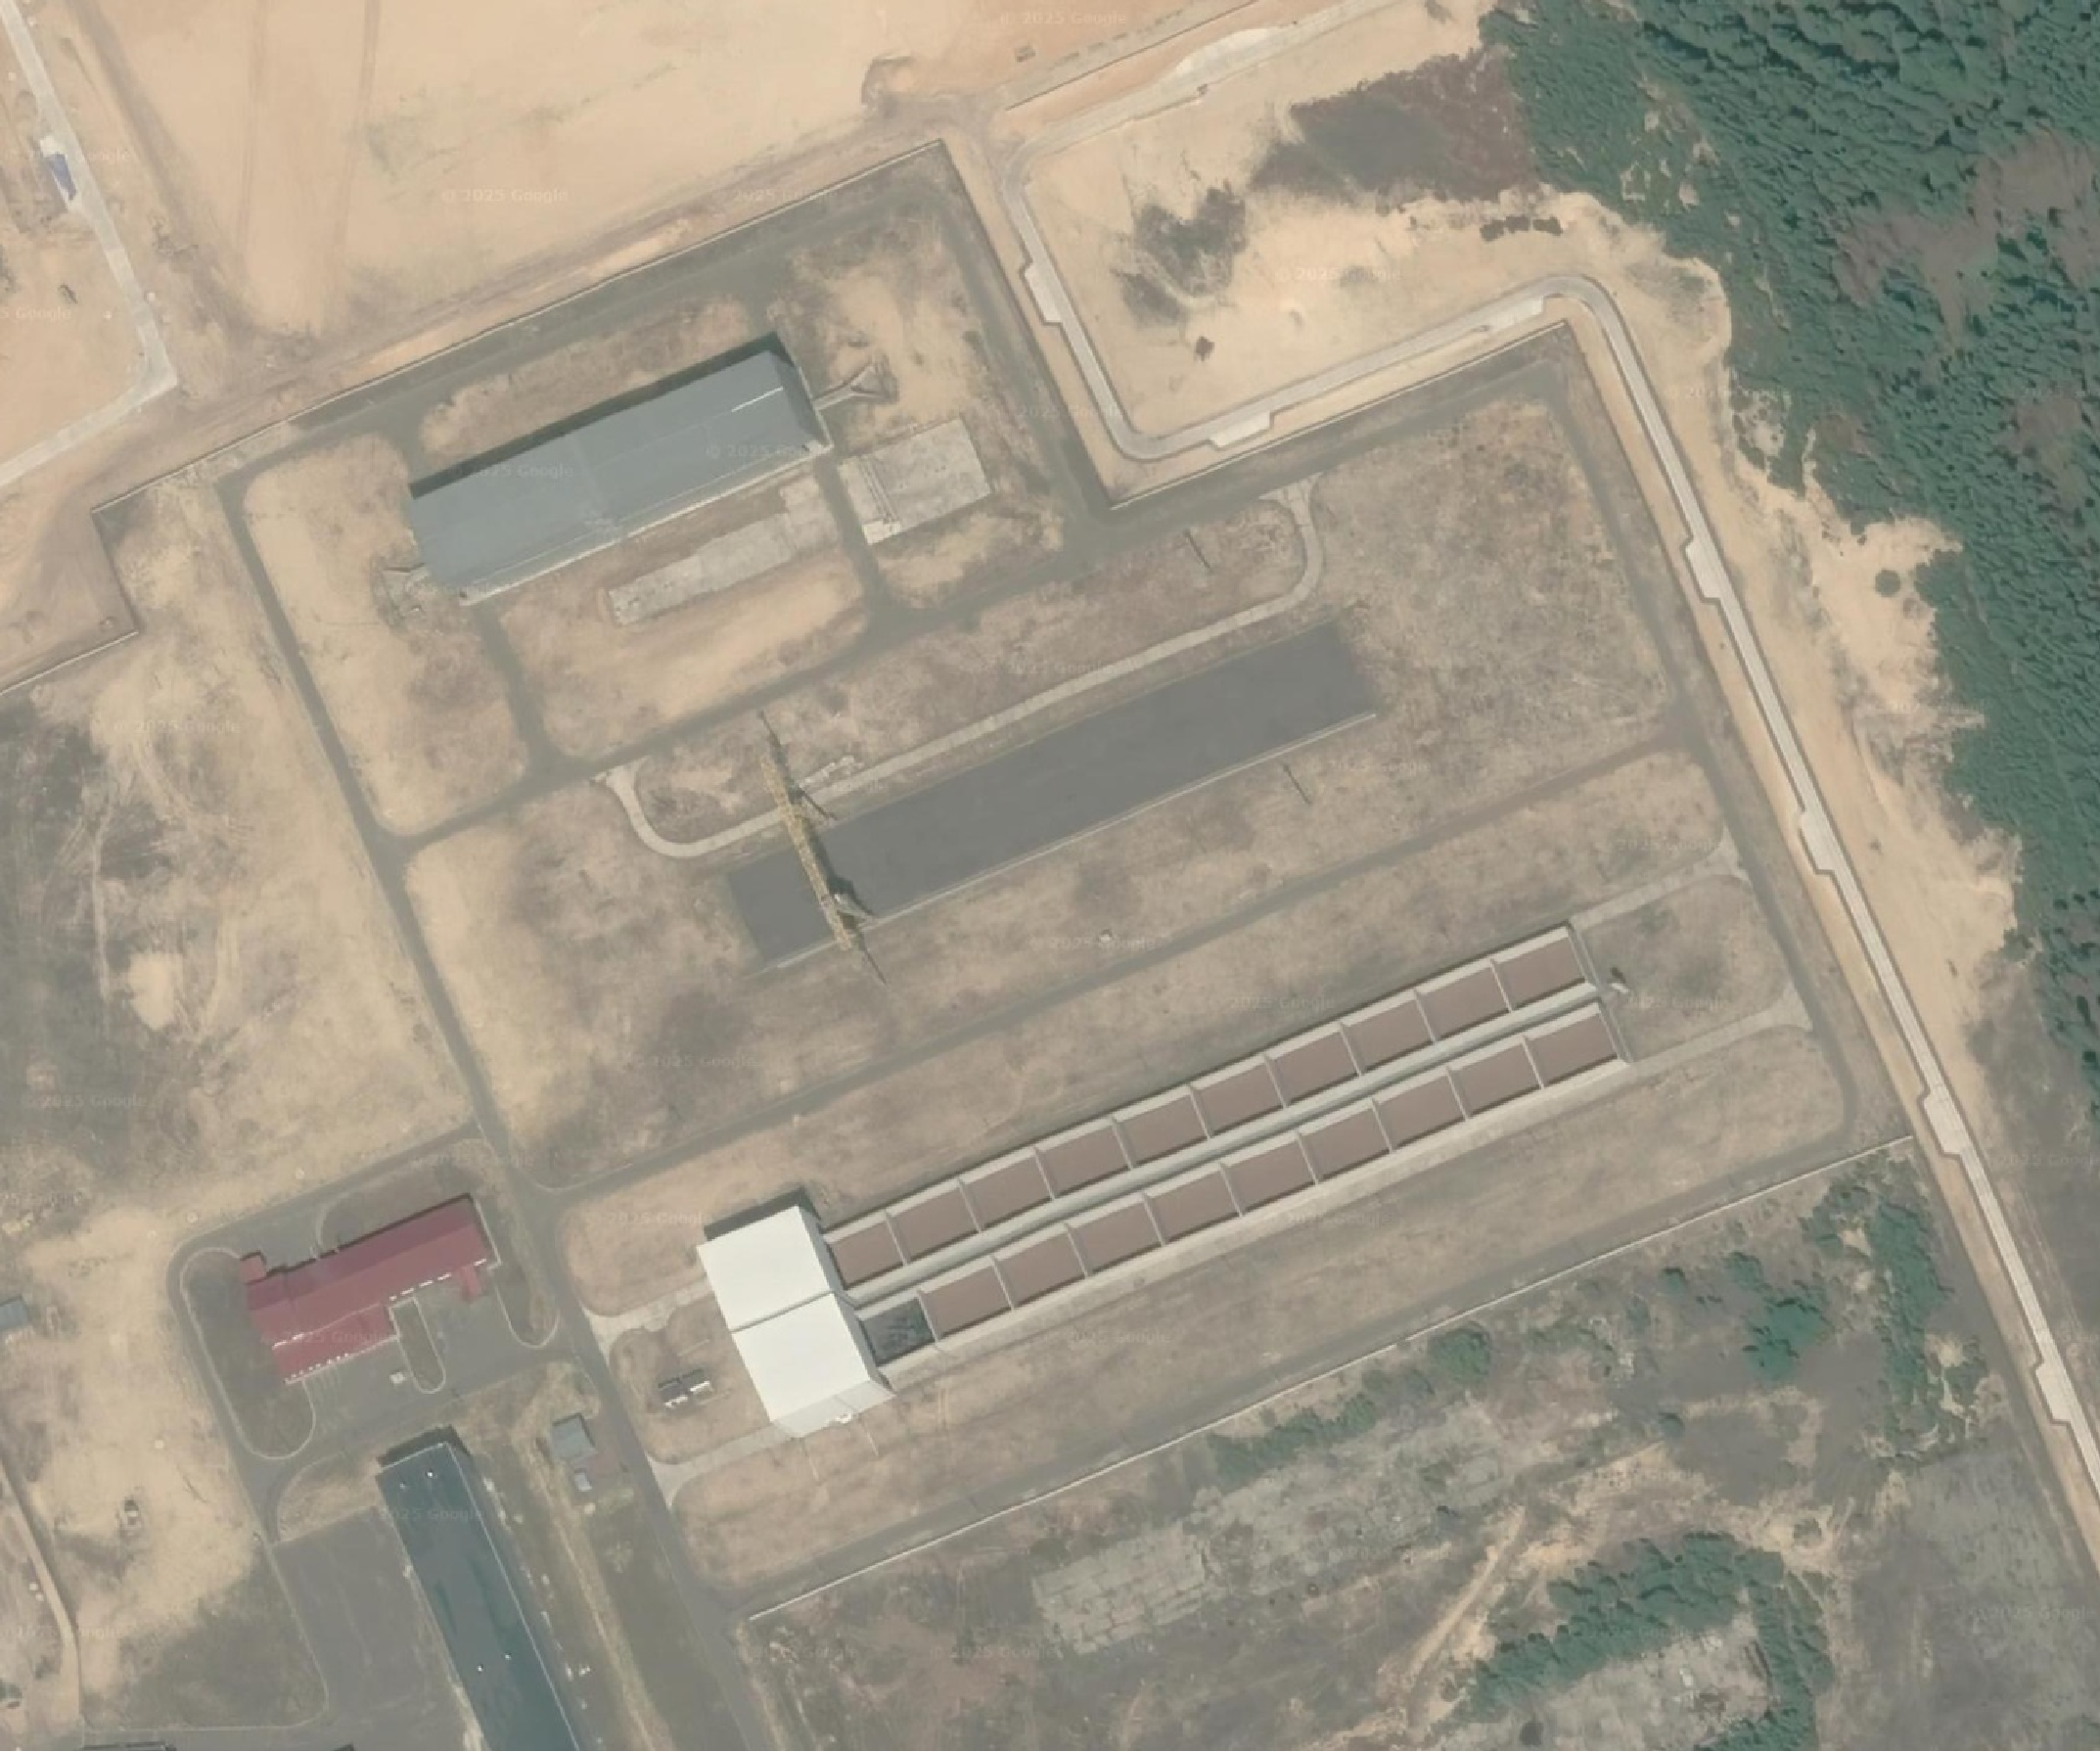
\includegraphics[width=0.45\textwidth]{figs/Jihwan/map1.pdf} &
        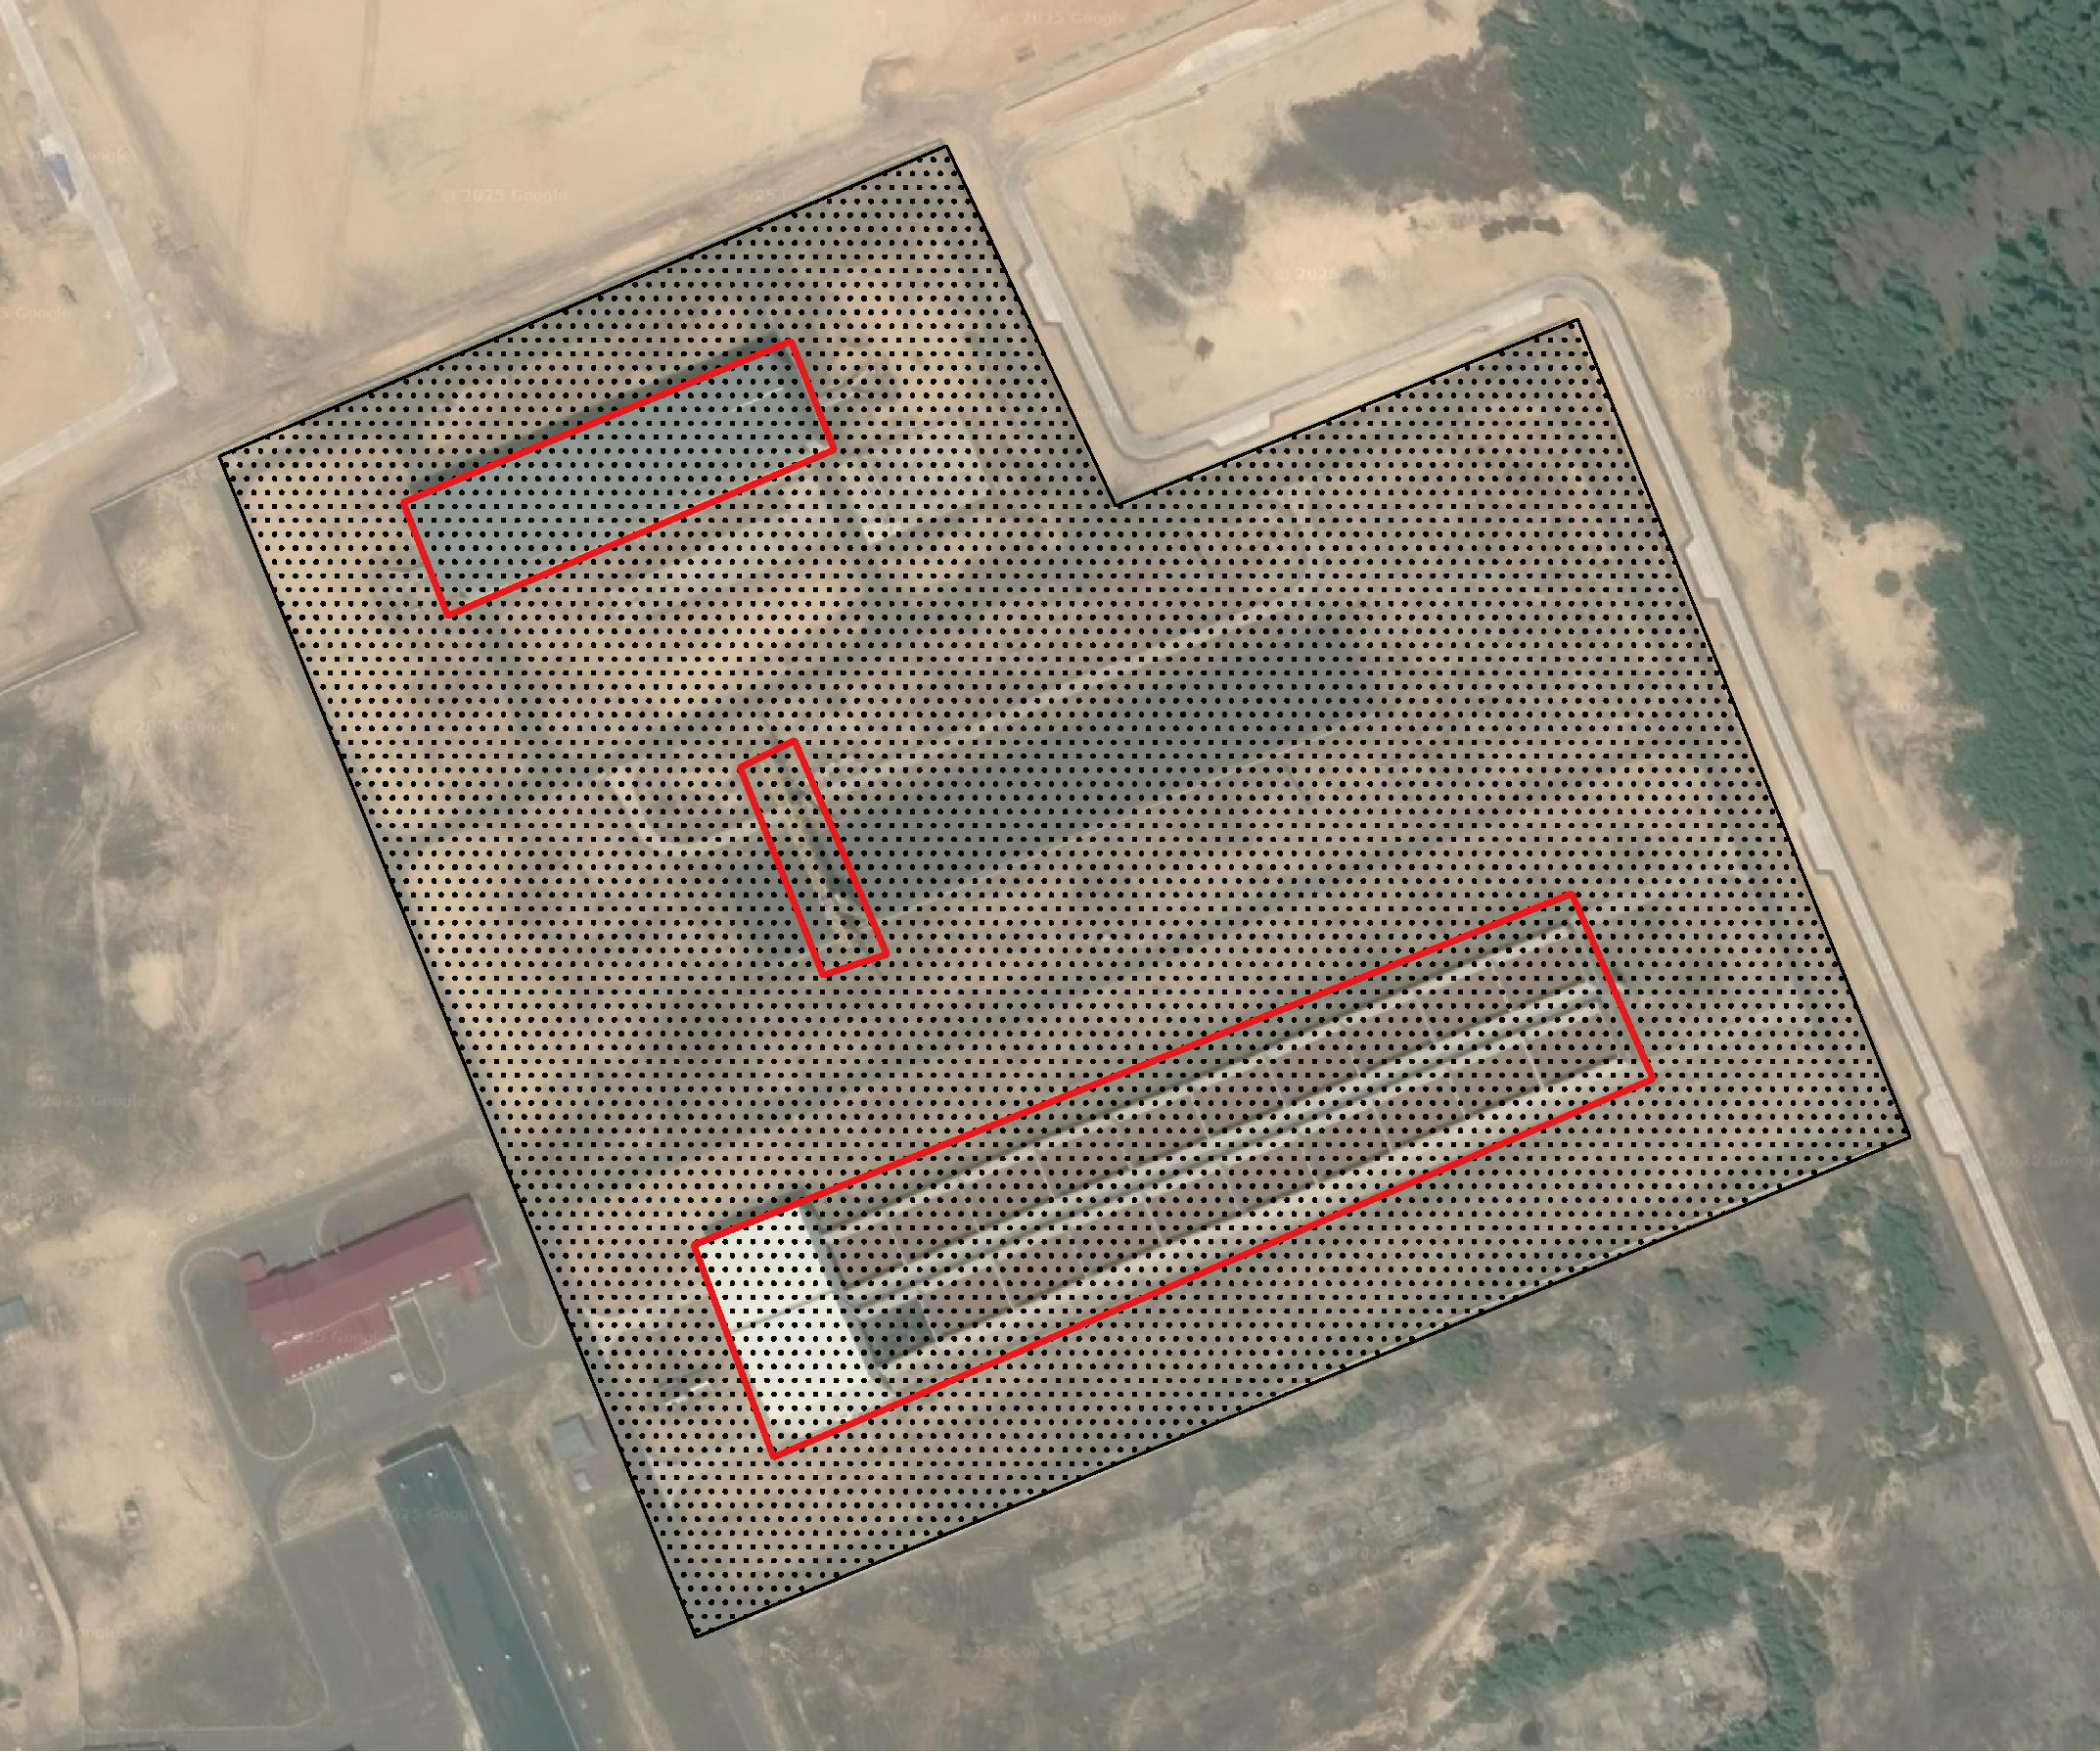
\includegraphics[width=0.45\textwidth]{figs/Jihwan/map2.pdf} \\
        (a) & (b) \\[10pt]
        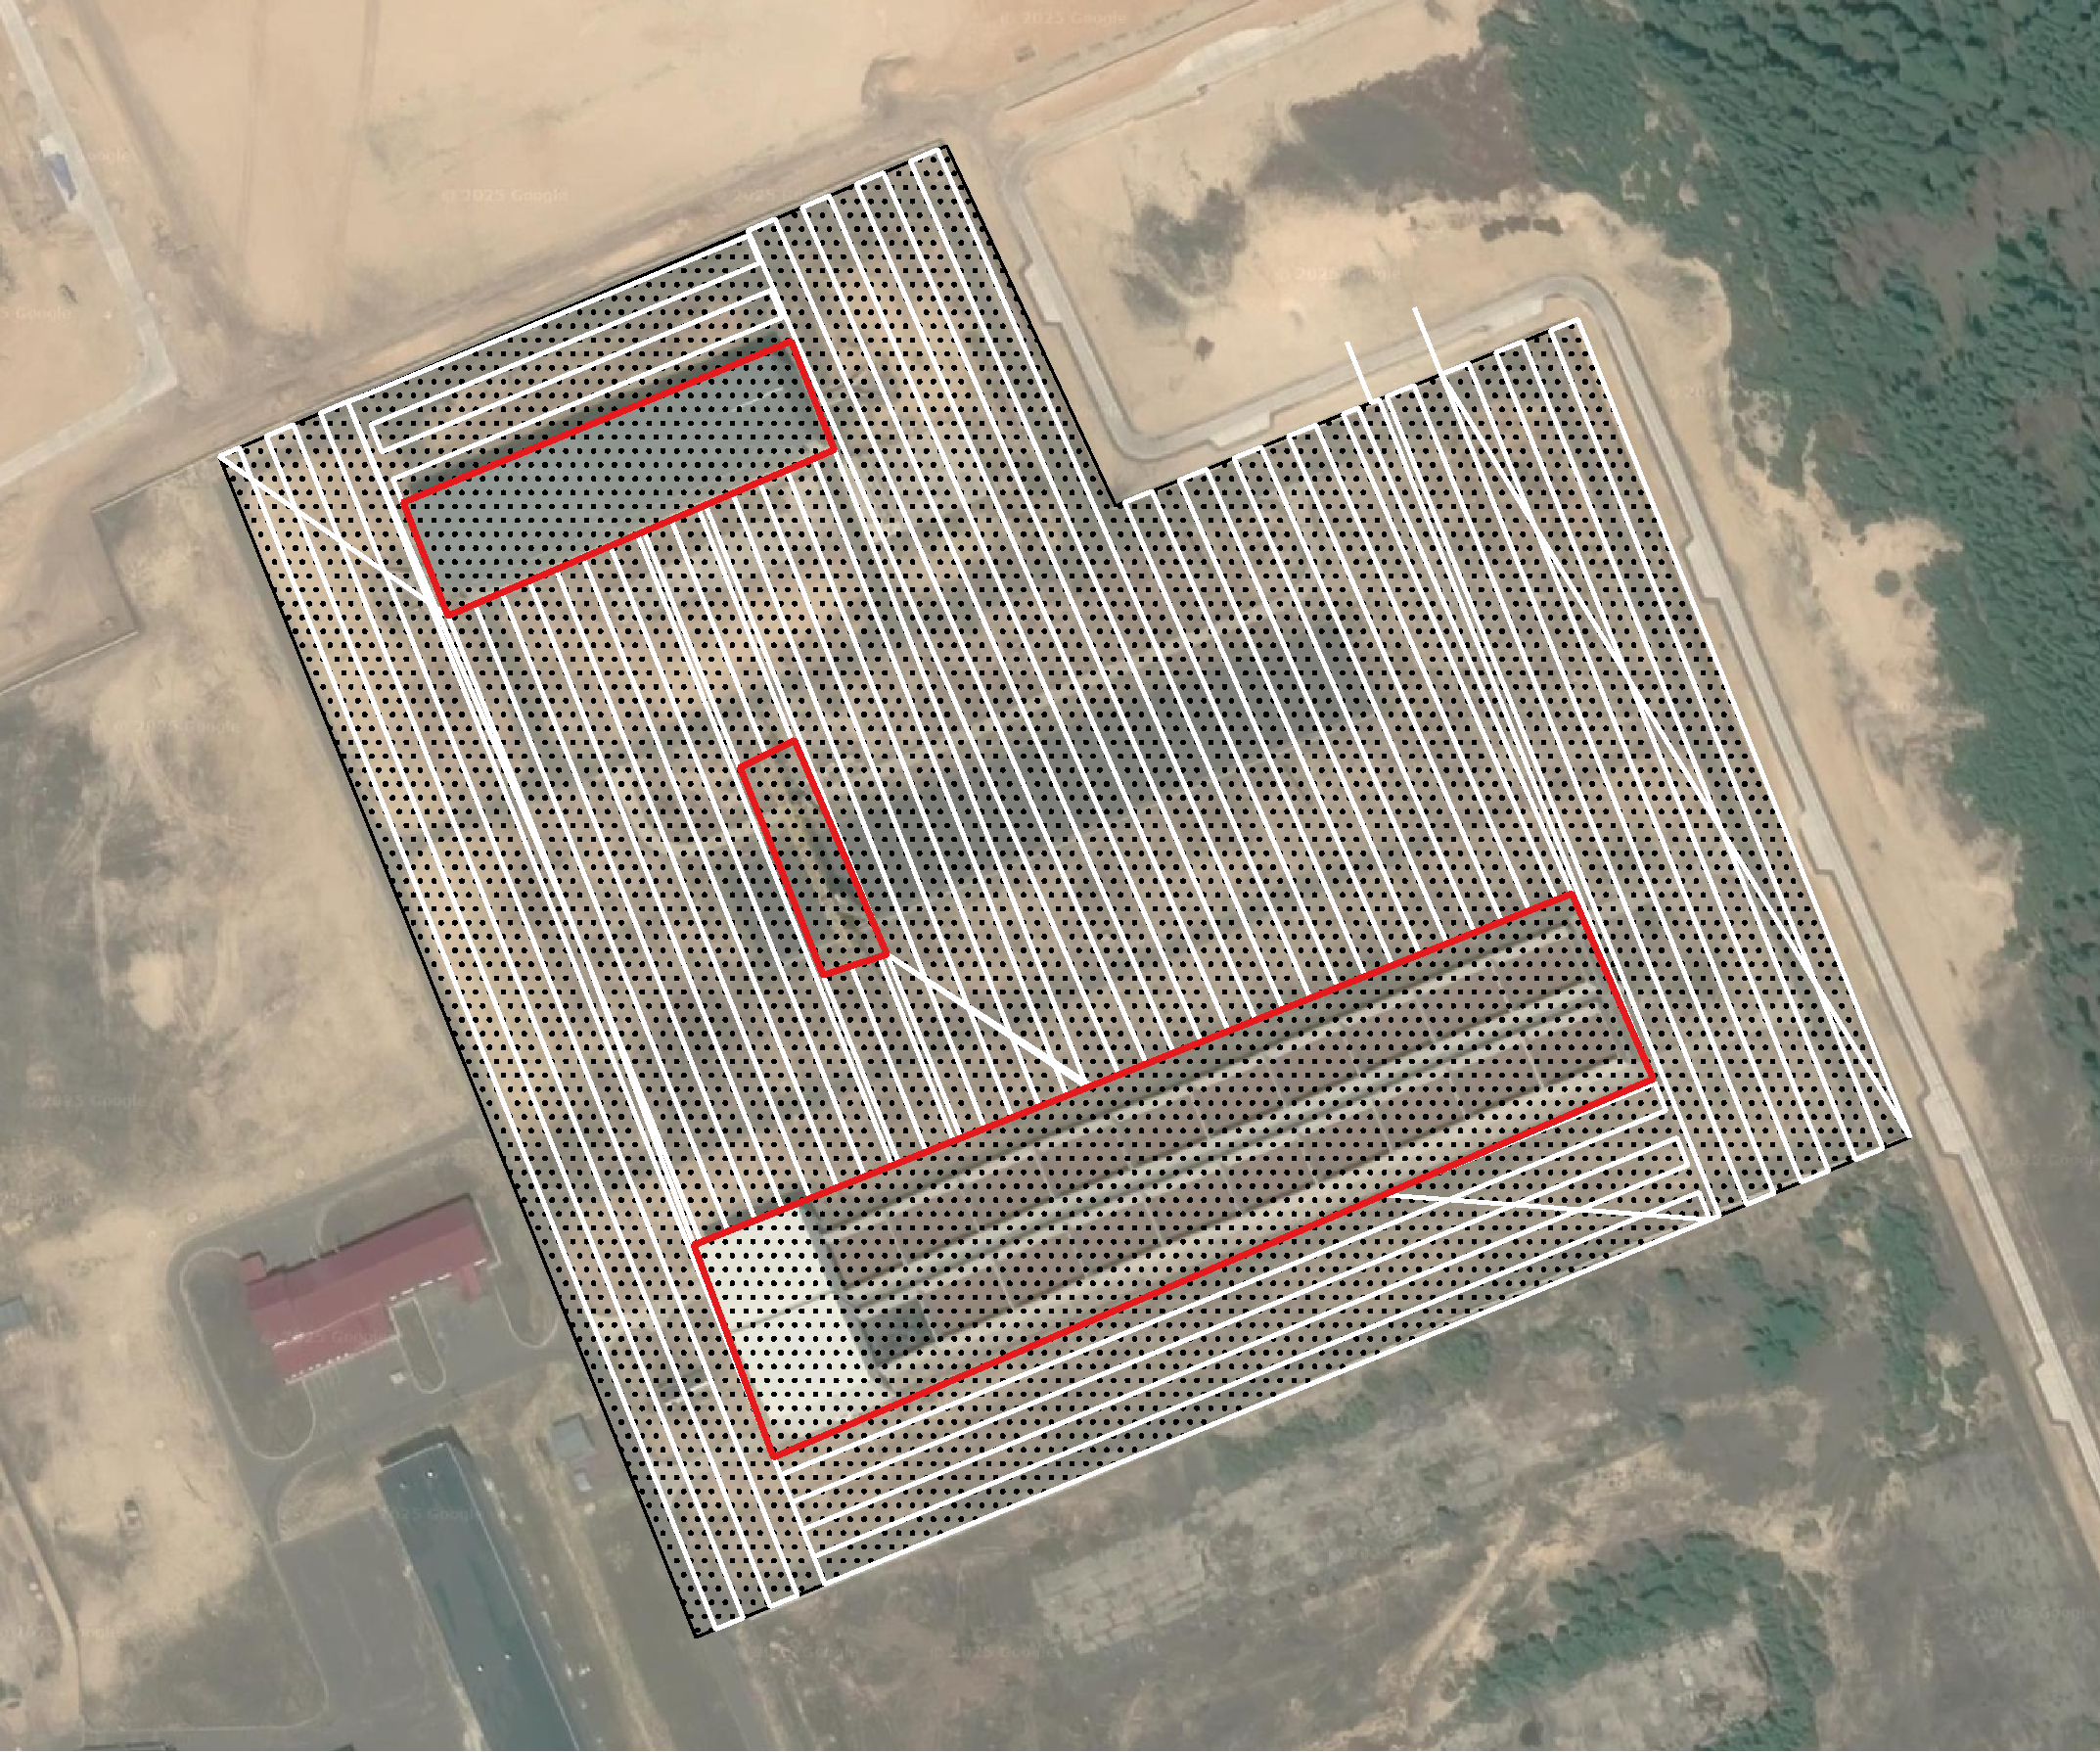
\includegraphics[width=0.45\textwidth]{figs/Jihwan/map3.pdf} &
        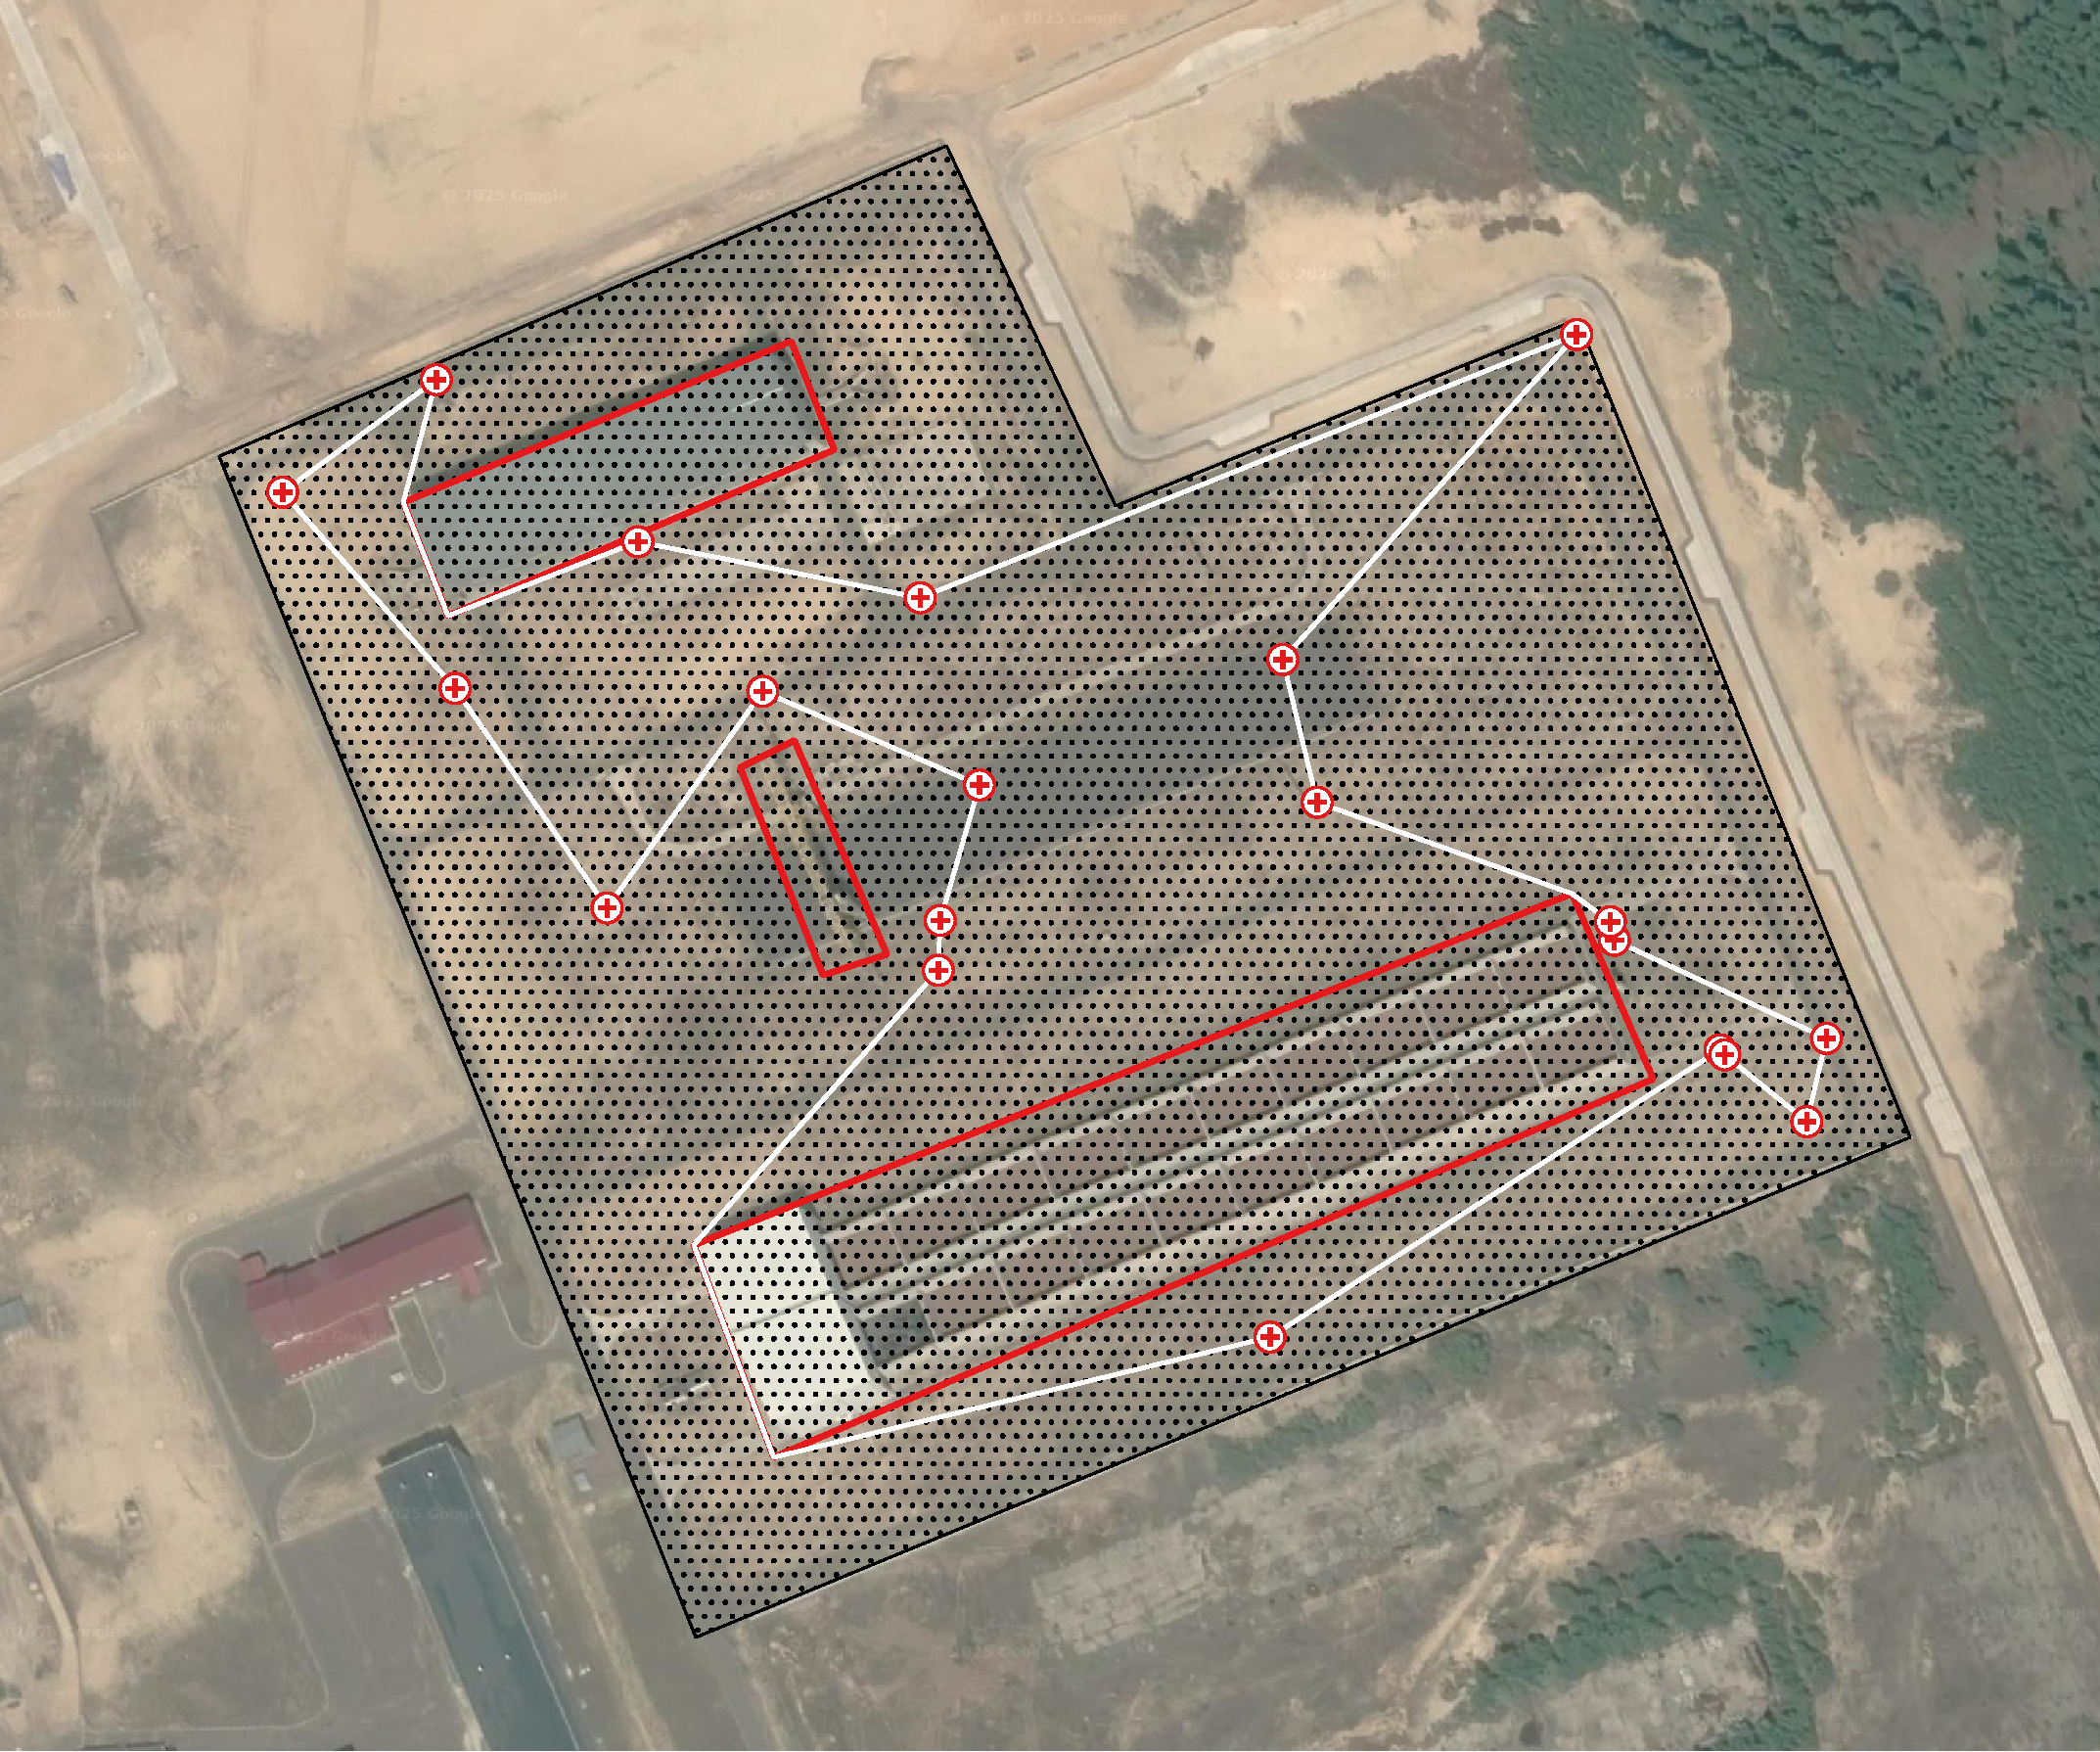
\includegraphics[width=0.45\textwidth]{figs/Jihwan/map4.pdf} \\
        (c) & (d)
    \end{tabular}
    \caption[Real Location Example for Mission Planning]
    {Real location example for generating a mission plan of a \gls{roi}. (a) The satellite view of a field in Ukraine. (b) The outer polygon (black dotted region) and holes (red regions) are drawn on \gls{qgis} to define the \gls{roi}. (c) The \gls{cpp} algorithm is executed to generate the thermal sensor drone path plan. (d) The \gls{tspo} algorithm is executed with 20 suspected landmine points to generate the \gls{GPR} sensor drone path plan. 
    }
    \label{fig:msp_example}
\end{figure}

%%%%%%%%%%
\subsection{Expanding to a Multi-Drone Operation}
\label{sec:msp_multi_drone}

Thus far, the mission planning algorithm has been explored for a single-drone operation. To make the system expandable, we must consider how to deploy a multi-drone system using the mission planning algorithm explained above. To do so, we introduce the Divide and Cluster method (based on \cite{skorobogatov2021multi}) for this problem. The method starts by dividing the \gls{roi} into smaller cells, which then get clustered into subregions that can be surveyed by individual drones adopting the layered approach.

\subsubsection{Divide and Cluster}

\paragraph{Divide} To divide the \gls{roi}, we can use triangulation algorithms which generate a mesh of triangles for a given set of vertices. In particular, we apply the \gls{cdt} from \gls{cgal} 2D Triangulations package \cite{cgal2024triangulation} to the \gls{roi}. Delaunay triangulation generates triangles which must conform to the Delaunay property: the circumcircle of a triangle must not include any other vertices than the triangle itself. \gls{cdt} is a variation in which pre-defined edges (i.e. the edges of the \gls{roi}) must be included in the final triangulation, while allowing some relaxation in the Delaunay property. The result of applying \gls{cdt} to an example Polygon with Holes is shown in Figure~\ref{fig:msp_cdt}. 

\begin{figure}[h!]
    \centering
    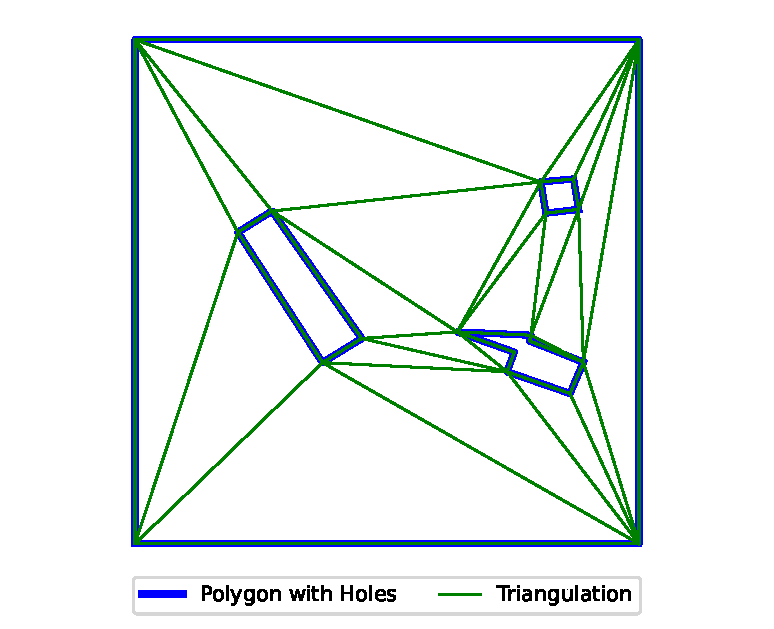
\includegraphics[width=0.6\linewidth]{figs/Jihwan/cdt.pdf}
    \caption[Constrained Delaunay Triangulation of Polygon with Holes]
    {The \gls{cdt} of a Polygon with Holes has been generated using \gls{cgal}'s 2D Triangulations package.}
    \label{fig:msp_cdt}
\end{figure}

\paragraph{Cluster} The divided mesh should now be clustered to form $n$ subregions that are each covered by a drone. The resulting subregions should meet 2 requirements: high compactness ($\mathrm{Compactness} = \frac{\mathrm{Area}}{\mathrm{Perimeter}}$ is maximised to generate a more efficient \gls{bcd} path) and similarity in area (so that each drone gets a fair share which allows us to deploy the least number of drones). Possible options for the clustering algorithm include methods based on region-growing (seed triangles are allocated and grow into adjacent triangles until $n$ subregions remain, similarly to \cite{skorobogatov2021multi}) and METIS \cite{karypis1997metis} (multi-level graph partitioning algorithm can be applied on the mesh), which need to be implemented and tested for validation. 

The Divide and Cluster method is visualised by Figure~\ref{fig:msp_divide_cluster} where the clusters have been manually allocated to demonstrate the idea in theory. A real implementation of the clustering algorithm will need to be made to fully validate the method in practice. 

\begin{figure}[h!]
    \centering
    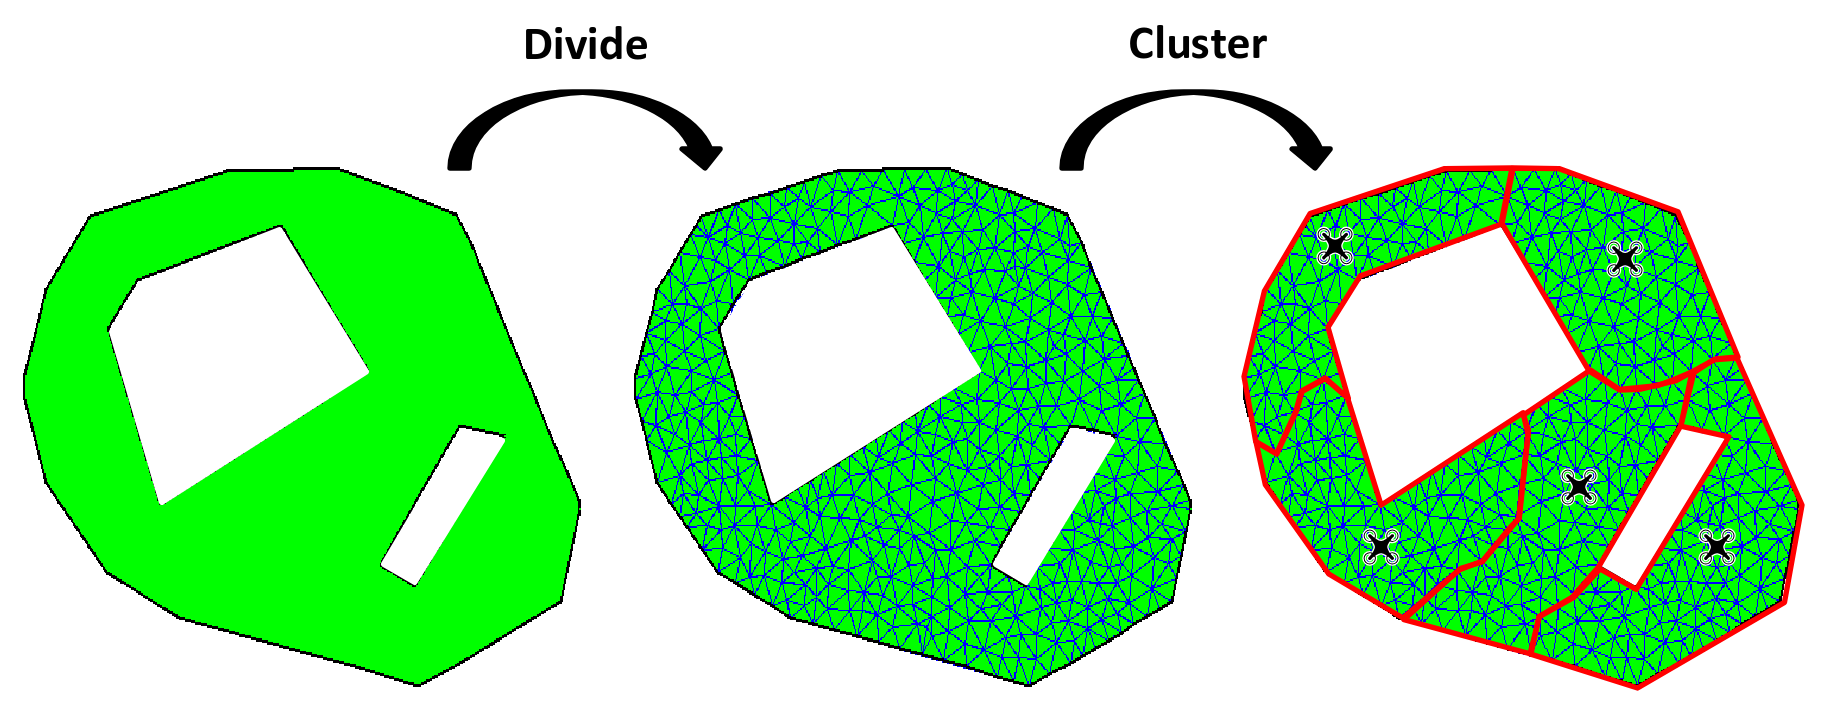
\includegraphics[width=\linewidth]{figs/Jihwan/Divide and Cluster.png}
    \caption[Divide and Cluster Method]
    {Divide and Cluster method visualised. A Polygon with Holes is divided using constrained Delaunay triangulation, then clustered into 5 subregions which can each be covered by a drone adopting the layered approach. The Polygon with Holes and the triangulation have been adopted from an example by \cite{cgal2024triangulation}.}
    \label{fig:msp_divide_cluster}
\end{figure}

\subsubsection{Possible Alternatives and Improvements}

\paragraph{Line Division} Instead of the Divide and Cluster method, the \gls{roi} may be directly decomposed into $n$ subregions of equal area using $n-1$ parallel line segments. This offers algorithm simplicity and greatly reduced computation times, but it is more likely to generate inefficient coverage paths as the compactness requirement is not considered. 

\paragraph{Boustrophedon Division} \gls{bcd} algorithm could be used during the Divide stage instead of \gls{cdt}, which would result in more appropriate polygons for generating boustrophedon coverage paths. However, \gls{bcd} tends to generate a smaller number of cells than \gls{cdt} which may make it harder to achieve the compactness and area requirements.  

\paragraph{Constrained Conforming Delaunay Triangulation} The example of \gls{cdt} in Figure~\ref{fig:msp_cdt} shows irregularly shaped and sized triangles being formed, which makes it harder to achieve the compactness and area requirements. \cite{shewchuk1996triangle} provides an implementation of the \gls{ccdt} which can be used to generate a more ideal mesh as demonstrated in Figure~\ref{fig:msp_shewchuk}. Additional software will need to be written to apply the algorithm to our \gls{cgal} Polygon with Holes object. 

\begin{figure}[h!]
    \centering
    \begin{tabular}{p{0.3\textwidth}p{0.3\textwidth}p{0.3\textwidth}}
        
\includegraphics[width=0.3\textwidth]{figs/Jihwan/triangulation_original.png} &
        
\includegraphics[width=0.3\textwidth]{figs/Jihwan/triangulation_cdt.png} &
        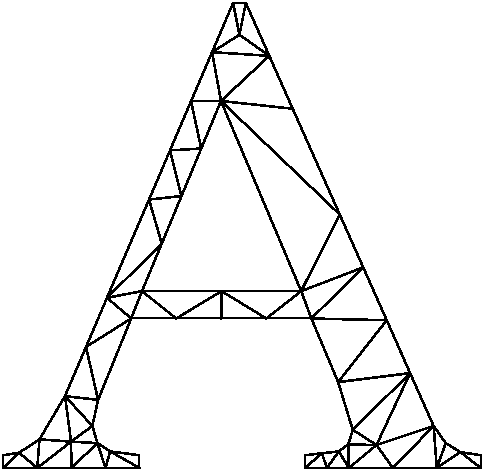
\includegraphics[width=0.3\textwidth]{figs/Jihwan/triangulation_ccdt.png} \\
        \centering (a) The letter A (\gls{roi}). & 
        \centering (b) After applying \gls{cdt}. & 
        \centering (c) After applying \gls{ccdt}.
    \end{tabular}
    \caption[Comparison of Triangulation Methods]
    {Comparison of \gls{cdt} and \gls{ccdt} applied to the letter A, taken from \cite{shewchuk1996triangle}.}
    \label{fig:msp_shewchuk}
\end{figure}


%%%%%%%%%%
\subsection{Comparison with Previous Landmine Detection Systems}
\label{sec:msp_comparison_manual_demining}

\subsubsection{Efficiency}

To evaluate the efficiency of the landmine detection system, we can compare the coverage time per unit area ($\varepsilon$). The expressions for the layered, magnetic-sensor (a commonly used option for aerial landmine detection systems) and manual approaches are shown in Equations \ref{eq:msp_layeredefficiency}, \ref{eq:msp_magneticefficiency} and \ref{eq:msp_manualefficiency} respectively using symbols explained in Table \ref{tab:msp_efficiencyvariables}.
\begin{equation}
\label{eq:msp_layeredefficiency}
\varepsilon_{\mathrm{layered}} = \frac{\frac{C_{\mathrm{thermal}}}{v_{\mathrm{thermal}}}+\frac{T_{\mathrm{GPR}}}{v_{\mathrm{GPR}}}}{A_{\mathrm{ROI}}}
\end{equation}
\begin{equation}
\label{eq:msp_magneticefficiency}
\varepsilon_{\mathrm{magnetic}} = \frac{\frac{C_{\mathrm{magnetic}}}{v_{\mathrm{magnetic}}}}{A_{\mathrm{ROI}}}
\end{equation}
\begin{equation}
\label{eq:msp_manualefficiency}
\varepsilon_{\mathrm{manual}} = \frac{t_{\mathrm{manual}}}{A_{\mathrm{ROI}}}
\end{equation}

\begin{table}[h!]
    \centering
    \begin{tabular}{|c|p{0.5\linewidth}|c|}
    \hline
        \textbf{Symbol} & \textbf{Explanation} & \textbf{Unit} \\
    \hline\hline
        $\varepsilon_{\mathrm{method}}$ & Coverage time per unit area of the given method. & $\mathrm{s} \, \mathrm{m}^{-2}$ \\
    \hline
        $C_{\mathrm{sensor}}$ & Length of the coverage path generated using \gls{bcd} algorithm for the coverage width of the given sensor.  & $\mathrm{m}$ \\
    \hline
        $v_{\mathrm{sensor}}$ & Maximum flight speed of the drone attached with the given sensor. & $\mathrm{m} \, \mathrm{s}^{-1}$ \\
    \hline
        $T_{\mathrm{GPR}}$ & Length of the target path generated using \gls{tspo} algorithm that should be surveyed using the \gls{GPR} sensor. & $\mathrm{m}$ \\
    \hline
        $t_{\mathrm{manual}}$ & Time taken for the \gls{roi} to be fully covered using manual detection methods. & $\mathrm{s}$ \\
    \hline
        $A_{\mathrm{ROI}}$ & Area of the \gls{roi}. & $\mathrm{m}^{2}$ \\
    \hline
    \end{tabular}
    \caption[Explanation of Variables for Mission Efficiency Expressions]
    {Explanation of the variables used in Equations \ref{eq:msp_layeredefficiency}, \ref{eq:msp_magneticefficiency} and \ref{eq:msp_manualefficiency} to express the mission efficiency.}
    \label{tab:msp_efficiencyvariables}
\end{table}

$C_{\mathrm{sensor}}$, $v_{\mathrm{sensor}}$ and $T_{\mathrm{GPR}}$ are dependent on the specifications of the sensors as well as the geometry of the \gls{roi}. The main difference in $\varepsilon_{\mathrm{layered}}$ and $\varepsilon_{\mathrm{magnetic}}$ rise from the small coverage width of a magnetic sensor compared to a thermal sensor. \cite{Yoo2024UnmannedAV} suggests a coverage width (survey interval) of 1\,m for a landmine detection drone using a magnetic sensor compared to 9\,m for our thermal sensor, which would significantly increase $C_{\mathrm{sensor}}$ (similarly to Figure~\ref{fig:msp_bahnemann}). Most of the parameters could not be found in related works on thermal, \gls{GPR} and magnetic sensor equipped drones -- real world experiments will need to be conducted with fine-tuning to find their values achieving the best results. \cite{gichd2005manual} states that manual mine clearance (with ground penetration) range between 12.5 and 125\,m$^2$ per deminer per day in terms of efficiency. The value includes both detection and removal. 

\subsubsection{Expandability}

In manual mine detection systems, additional human resources should be added to cover a larger area of land which is both costly and difficult to obtain. The proposed mission planning framework greatly improves the expandability by utilising the multi-aerial drone system with the Divide and Cluster method, allowing the operator to survey larger areas by deploying additional drones and base stations. 

\subsubsection{Intuitiveness}

The layered approach offers an intuitive solution by incorporating the \gls{qgis} interface and automatic path planning algorithms which can be used even by inexperienced operators in demining organisations. The system also returns the analysed data in a more interpretable format through \gls{qgis} maps, which helps the demining organisations plan future missions more efficiently.

%%%%%%%%%%
\subsection{Limitations}
\label{sec:msp_limitations}

To further improve the mission planning framework, some of its limitations are listed below along with suggestions on how they can be mitigated. 

\subsubsection{Manually Labelled Region of Interest}

In the Define step of the layered approach, the operator must manually label the outer boundary and obstacles of the \gls{roi} using the polygon tool in \gls{qgis}. This becomes a time-consuming task as more vertices are introduced, and the manual procedure also introduces an inconsistency in the definition of the \gls{roi}. If multiple operators work on defining the obstacles in a large \gls{roi}, the offset required for safe maneuver by the drones may differ. 

As a solution, image segmentation algorithms can be implemented to partially automate this process. Image segmentation models like Segment Anything Model 2 \cite{ravi2024sam2} can be used to automatically identify the vertices of obstacles which can be selected and adjusted by the operator. 

\cite{patil2022segment} proposes a more specialised semantic segmentation model to automatically segment satellite images into regions and identify its class (building, land, road, vegetation, water, or miscellaneous). This can speed up the progress of defining the \gls{roi} by removing areas such as bodies of water and buildings which are unlikely to be populated by landmines. 

\subsubsection{Use of Satellite Image Databases}
\label{sec:msp_satellite_database_limitation}

The current mission planning framework uses openly available satellite databases during the Define step of the layered approach. However, outdated satellite images may result in missing out newly introduced or removed obstacles in the \gls{roi}. 

Mine Kafon\footnote{\url{https://minekafon.org/}} deploys a lightweight mapping drone (MK Destiny) to automatically generate the 3D map of the \gls{roi}. The \gls{cpp} algorithm could be modified to deploy a drone equipped with RGB camera to map the \gls{roi} in a similar way.  

\subsubsection{Streamlining the User Interface}

The \gls{cpp} and \gls{tspo} algorithms are not directly connected to the \gls{qgis} interface; currently, the user must manually import and export the \gls{roi} and path plans as a GeoJSON format before and after running the C++ scripts. 

\gls{qgis} allows developers to create custom Python plugins to add additional functionalities to the interface. By wrapping the \gls{cpp} and \gls{tspo} algorithms \gls{qgis} plugins, the operator will be able to easily run these algorithms within the interface without having to compile or run C++ scripts on their own. 

\subsubsection{Testing in Real World Scenarios}

In this report, the mission planning framework was tested for a real location example in Figure~\ref{fig:msp_example}. However, the example does not fully demonstrate a real multi-aerial drone system using the Divide and Cluster method.

Real world testing will need to be conducted for a variety of different \gls{roi} locations (with varying terrains, soil composition, weather conditions, etc.), evaluating the efficiency of the proposed mission planning framework. This will help to create a robust system that can easily be applied across different regions and scenarios. 